\documentclass[10pt,a4paper]{article}
\usepackage{amsmath, amsfonts, amssymb}
\usepackage[utf8]{inputenc}
\usepackage[OT1]{fontenc}
\usepackage{gensymb}
\usepackage[margin=2.5cm, landscape]{geometry}
\usepackage{graphicx}
\usepackage[dvipsnames]{xcolor}
\usepackage{paracol}
\usepackage{calc}
\usepackage{enumitem}
\usepackage[hang, font ={small, it}, labelformat=empty]{caption}
\renewcommand{\figurename}{Fig}

\usepackage[object=vectorian]{pgfornament}

\usepackage{tikz}
\usepackage[uprightgreeks,frenchstyle,light,fulloldstylenums,veryoldstyle]{kpfonts}

\globalcounter{enumi}
\newcommand{\switchenum}{\setcounter{enumi}{\arabic{enumi}-1}\switchcolumn}
\renewcommand{\theenumi}{\S.\arabic{enumi}}

\setlength{\parskip}{1ex}
\setlength{\parindent}{0pt}

\DeclareMathOperator{\tang}{tang.}
\DeclareMathOperator{\cotg}{cot.}
\DeclareMathOperator{\sing}{sin.}
\DeclareMathOperator{\cosg}{cos.}

\pagestyle{empty}

\def\D{\mathrm{d}}

\renewcommand{\rmdefault}{cmr}

\begin{document}
	
	\begin{paracol}{2}
	\par \textit{Nova Acta Eruditorum 1745, p. 523}
	\par E79 (Eneström Index) 
	\begin{center}
		\par \pgfornament[width = 0.8\linewidth]{88}
		
		\par {\bf Problema geometricum, propositum}\\
		publice ab anonymo geometra
	\end{center}
	\switchcolumn
	\par \textit{Nova Acta Eruditorum 1745, p. 523}
	\par E79 (Eneström Index) 
	\begin{center}
		\par \pgfornament[width = 0.8\linewidth]{88}
		
		\par {\bf Voorstel tot een meetkundig probleem}\\
		publiek door een anomnieme meetkundige
	\end{center}
	\switchcolumn*
	
	
	\par Proposito puncto $F$ invenire omnes curves $AMBN$ huius naturae, ut singuli radii ex $F$ egressi post duplicem reflectionem in $M$ \& $N$ in idem punctum $F$ revertantur.  Primum quidem perspicuum est omnes ellipses, quae in $F$ habeant alterutrum focum, quaesito satisfacere.  Sed praeterea dantur innumerabiles aliae curvae, eadem indole gaudentes, quarum investigatio limites analyseos non parum extendere videtur.
		
	\switchcolumn
	\par Gegeven een punt $F$, vind alle krommen $AMBN$ zodat, elke straal vanuit $F$, na twee terugkaatsingen in $M$ \& $N$, terug in het originele punt $F$ terechtkomt. Een eerste van zo'n soort krommen zijn alle ellipsen, die een brandpunt hebben in het punt $F$. Maar er kunnen ontelbaar veel andere krommen gegeven worden die dezelfde eigenschap hebben, de wijze om deze analytisch te onderzoeken is nog niet gezien.

	\switchcolumn*
			
	\begin{figure}[h]
		\centering
		\par {
			\fontfamily{jkplvos}\selectfont
			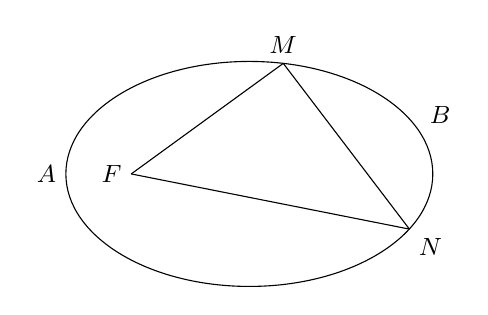
\begin{tikzpicture}[yscale=0.8]
			\draw [rotate around={0:(1.5,0)}] (1.5,0.) ellipse (2.33cm and 1.786cm);
			\draw (0,0)-- (1.931,1.755);
			\draw (1.931,1.755)-- (3.533,-0.876);
			\draw (3.5330,-0.876)-- (0,0);
			\draw (0,0) node [left] {\small $F$};
			\draw (1.93,1.75) node [above] {\small $M$};
			\draw (3.53,-0.87) node [below right] {\small $N$};
			\draw (-0.83,0) node [left] {\small $A$};
			\draw (3.67,0.64) node [above right] {\small $B$};
			\end{tikzpicture}}
		\fontfamily{cmr}\selectfont
		\caption{Tab. III. Fig. 3.}
	\end{figure}
	\switchcolumn
	\begin{figure}[h]
		\centering
		\par {
			\fontfamily{jkplvos}\selectfont
			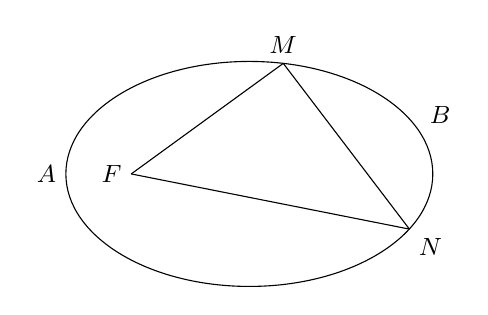
\begin{tikzpicture}[yscale=0.8]
			\draw [rotate around={0:(1.5,0)}] (1.5,0.) ellipse (2.33cm and 1.786cm);
			\draw (0,0)-- (1.931,1.755);
			\draw (1.931,1.755)-- (3.533,-0.876);
			\draw (3.5330,-0.876)-- (0,0);
			\draw (0,0) node [left] {\small $F$};
			\draw (1.93,1.75) node [above] {\small $M$};
			\draw (3.53,-0.87) node [below right] {\small $N$};
			\draw (-0.83,0) node [left] {\small $A$};
			\draw (3.67,0.64) node [above right] {\small $B$};
			\end{tikzpicture}}
		\fontfamily{cmr}\selectfont
		\caption{Tab. III. Fig. 3.}
	\end{figure}

	\newpage
	\switchcolumn*
			
	\par \textit{Acta Academia Scientiarum Imperialis Petropolitanae 1778, p. 3}
	\par E513 (Eneström Index) 
	\begin{center}
		\par \pgfornament[width = 0.8\linewidth]{88}
		
		\par {\bf De curvis triangularibus}\\
		Autore\\
		\textsc{L. Euler}
	\end{center}
	\switchcolumn
	
	\par \textit{Acta Academia Scientiarum Imperialis Petropolitanae 1778, p. 3} 
	\par E513 (Eneström Index) 
	\begin{center}
		\par \pgfornament[width = 0.8\linewidth]{88}
		
		\par {\bf Over de driehoekige krommen}\\
		Auteur\\
		\textsc{L. Euler}
	\end{center}
	\switchcolumn*

	\par \begin{enumerate}[topsep=1px]
		\item Curvas triangulares voco, quae tribus arcubus $AB$, $AC$ et $BC$ intus inflexis constant, qui in angulis $A$, $B$ et $C$ coeant, praeterea autem nullos alios ramos contineant. Huiusmodi ergo curvae ut sint continuae, sive quapiam aequatione, vel algebraica, vel etiam transcendente, exprimi queant, necesse est, ut in angulis $A$, $B$ et $C$ habeant cuspides acutissimas, ubi bini arcus coeuntes communi tangente sint praediti. Tales autem curvas innumerabiles exhiberi posse, tam algebraicas, quam transcendentes, iam olim ostendi, cum Problema de eiusmodi curvis, circa datum punctum lucidum describendis, proposuissem, ita ut omnes radii, a curvua bis reflexi, iterum in ipsum punctum lucidum revertantur, quod Problema variis solutionibus in Actis Lipsiensibus pro Annis 1746 et 1748 solutum reperitur. Hic enim tota solutio ad inventionem huiusmodi curvarum triangularium reducitur, quippe quibus causticae radiorum reflexorum formantur. 
			
		\switchenum
		\item Ik noem driehoekige krommen, deze uit drie bogen $AB, AC$ en $BC$ naar binnen gebogen, die in de hoeken $A$, $B$ en $C$ samenkomen en die ook geen andere vertakkingen bevatten. Deze krommen van deze aard zijn continu en \textbf{kunnen uitgedrukt worden volgens zekere vergelijking}, hetzij algebraïsch, of zelfs transcendent, het is essentieel, dat ze in de hoeken $A$, $B$ en $C$ scherpe spitsen hebben, waar de twee bogen samenkomen bevatten ze een gemeenschappelijke raaklijn. Er kunnen ontelbare zulke krommen gemaakt worden, zowel algebraïsch als transcendent, een lange tijd geleden heb ik aangetoond dat Problemen van de soorten krommen, die een bepaald brandpunt beschrijven, te verklaren, waarbij elke straal tweemaal terugkaatst in de kromme en terugkeert naar hetzelfde brandpunt, voor het welke probleem meerdere oplossingen in Actis Lipsiensibus gedateerd 1746 en 1748 gevonden werden. Hier worden deze oplossingen herleid tot het vinden van driehoekige krommen, immers vormen deze een brandpunt waar elke straal in terugkaatst. 
		
		\switchcolumn*
		
		\begin{figure}[h]
			\centering
			\par {
				\fontfamily{jkplvos}\selectfont
				\begin{tikzpicture}[rotate=180, scale=1]
				\draw [shift={(-1.651,-2.108)}]  plot[domain=0.141:0.906,variable=\t]({1.*2.678*cos(\t r)+0.*2.677*sin(\t r)},{0.*2.678*cos(\t r)+1.*2.678*sin(\t r)});
				\draw [shift={(1,2.484)}]  plot[domain=4.330:5.095,variable=\t]({1.*2.678*cos(\t r)+0.*2.678*sin(\t r)},{0.*2.678*cos(\t r)+1.*2.678*sin(\t r)});
				\draw [shift={(3.651,-2.108)}]  plot[domain=2.235:3.001,variable=\t]({1.*2.678*cos(\t r)+0.*2.678*sin(\t r)},{0.*2.678*cos(\t r)+1.*2.678*sin(\t r)});
				\draw (0,0) node [below right] {\small $C$};
				\draw (2,0) node [below left] {\small $B$};
				\draw (1,-1.732) node [above] {\small $A$};
				\end{tikzpicture}}
			\fontfamily{cmr}\selectfont
			\caption{Tab. I. Fig. 1.}
		\end{figure}
		\switchcolumn
		\begin{figure}[h]
			\centering
			\par {
				\fontfamily{jkplvos}\selectfont
				\begin{tikzpicture}[rotate=180, scale=1]
				\draw [shift={(-1.651,-2.108)}]  plot[domain=0.141:0.906,variable=\t]({1.*2.678*cos(\t r)+0.*2.677*sin(\t r)},{0.*2.678*cos(\t r)+1.*2.678*sin(\t r)});
				\draw [shift={(1,2.484)}]  plot[domain=4.330:5.095,variable=\t]({1.*2.678*cos(\t r)+0.*2.678*sin(\t r)},{0.*2.678*cos(\t r)+1.*2.678*sin(\t r)});
				\draw [shift={(3.651,-2.108)}]  plot[domain=2.235:3.001,variable=\t]({1.*2.678*cos(\t r)+0.*2.678*sin(\t r)},{0.*2.678*cos(\t r)+1.*2.678*sin(\t r)});
				\draw (0,0) node [below right] {\small $C$};
				\draw (2,0) node [below left] {\small $B$};
				\draw (1,-1.732) node [above] {\small $A$};
				\end{tikzpicture}}
			\fontfamily{cmr}\selectfont
			\caption{Tab. I. Fig. 1.}
		\end{figure}

		\switchcolumn*
		
		\item Praeter eum usum autem, quem istiusmodi curvae triangulares in commemorato problemate catoptrico praestant, imprimis considerari merentur curvae, quae ex evolutione talis curvae triangularis $A B C$ nascuntur. Hunc in sinem vocemus longitudinem arcus $A B = c$, arcus $AC=b$ et arcus $BC=a$. Iam arcui $AB$ concipiatur filum applicatum, quod extra $A$ prolongetur usque in $F$, ita ut sit $AF=f$, et stilus in $F$ insertus promoveatur, donec arcus $AB$ fuerit evolutus, et filum perveniat in situm $Bg$, eritque $Bg = AF +$ arcu $AB = f+c$; tum motus stili continuetur et filum $Bg$ successive applicetur arcui $BC=a$, donec perveniat in $H$, eritque 
		
		\[
			BC+CH = Bg = f+c, \quad \text{unde sit} \quad CH = f+c-a;
		\]
		\par quo cum fuerit perventum, filum applicetur arcui $CA$, ubi notari convenit, perinde esse, sive arcus $CA$ maior sit, sive minor arcu $CB$; semper enim filum totum arcum $CA$ occupare debet. Iam motus stili ex $H$ continuetur in $f$ donec filum $fA$ cuspidem $A$ tanget, tum igitur erit 
		\[
			Af = CH + AC = f+c-a+b;
		\]
			
		\switchenum
		\item Afgezien van het gebruik van, het geven van krommen van een driehoekige aard bij de bepaling van het \textit{catoptrische} probleem, verdienen vooral de krommen, die als evolvente uit de driehoekige krommen $ABC$ geboren worden, beschouwd te worden. Hierbij zal ik de lengte van de boog benoemen als $AB = c$, boog $AC=b$ en boog $BC=a$. Bevestig nu een touw aan de boog $AB$, en verleng dit vanuit $A$ tot in $F$, zodat $AF=f$, en beweeg een pen ingebracht in $F$, tot de boog $AB$ ontwikkeld wordt, en de draad aankomt in positie $Bg$, en dus $Bg = AF + \text{ de boog } AB = f+c$; beweeg opnieuw de pen continu en bevestig opeenvolgend de draad $Bg$ aan de boog $BC=a$, tot het aankomt in $H$, en dan
		\[
			BC+CH = Bg = f+c, \quad \text{zodat het is dat} \quad CH = f+c-a;
		\]
		\par wanneer dit is bereikt, bevestig de draad aan de boog $CA$; waarbij we afspreken te noteren, als het is, dat de boog $CA$ langer is, of de kortere boog $CB$, dan zal de draad altijd de gehele boog $CA$ moeten innemen. Beweeg nu een pen uit $H$ continu tot in $f$, zodat de draad $fA$ de spits $A$ raakt, dan is het dat  
		\[
			Af = CH + AC = f+c-a+b;
		\]
		
		\switchcolumn*
		\begin{figure}[h]
			\centering
			\par {
				\fontfamily{jkplvos}\selectfont
				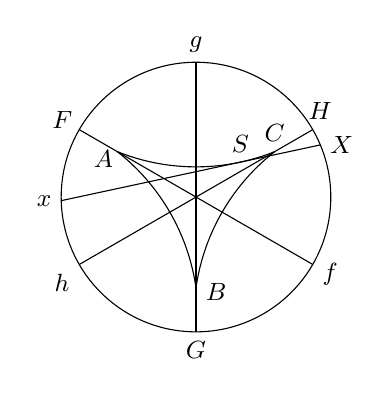
\begin{tikzpicture}
				\draw [shift={(-1.651,-2.108)}]  plot[domain=0.141:0.906,variable=\t]({1.*2.678*cos(\t r)+0.*2.677*sin(\t r)},{0.*2.678*cos(\t r)+1.*2.678*sin(\t r)});
				\draw [shift={(1,2.484)}]  plot[domain=4.330:5.095,variable=\t]({1.*2.678*cos(\t r)+0.*2.678*sin(\t r)},{0.*2.678*cos(\t r)+1.*2.678*sin(\t r)});
				\draw [shift={(3.651,-2.108)}]  plot[domain=2.235:3.001,variable=\t]({1.*2.678*cos(\t r)+0.*2.678*sin(\t r)},{0.*2.678*cos(\t r)+1.*2.678*sin(\t r)});
				\draw (1,-0.577) circle (1.712cm);
				\draw (1,1.135)-- (1,-2.290);
				\draw (2.483,-1.433)-- (-0.483,0.279);
				\draw (-0.483,-1.434)-- (2.483,0.279);
				\draw (2.579,0.085)-- (-0.712,-0.623);
				\draw (0,0) node [below left, yshift=4pt, xshift=2pt] {\small $A$};
				\draw (2,0) node [above] {\small $C$};
				\draw (1,-1.732) node [below right, yshift=5pt] {\small $B$};
				\draw (1,1.135) node [above] {\small $g$};
				\draw (2.483,0.279) node [above right, xshift=-5pt] {\small $H$};
				\draw (2.483,-1.434) node [below right, yshift=4pt] {\small $f$};
				\draw (-0.483,0.279) node [above left, yshift=-3pt, xshift=1pt] {\small $F$};
				\draw (-0.483,-1.434) node [below left] {\small $h$};
				\draw (1,-2.290) node [below] {\small $G$};
				\draw (1.563,-0.134) node [above] {\small $S$};
				\draw (2.579,0.085) node [right] {\small $X$};
				\draw (-0.712,-0.623) node [left] {\small $x$};
				\end{tikzpicture}}
			\fontfamily{cmr}\selectfont
			\caption{Tab. I. Fig. 2.}
		\end{figure}
		\switchcolumn
		\begin{figure}[h]
			\centering
			\par {
				\fontfamily{jkplvos}\selectfont
				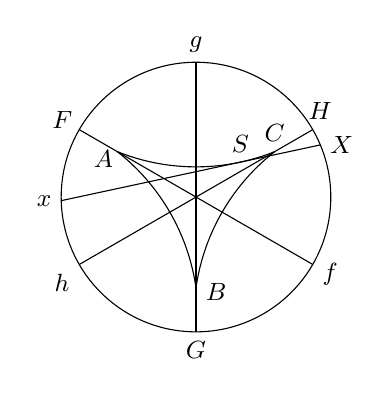
\begin{tikzpicture}
				\draw [shift={(-1.651,-2.108)}]  plot[domain=0.141:0.906,variable=\t]({1.*2.678*cos(\t r)+0.*2.677*sin(\t r)},{0.*2.678*cos(\t r)+1.*2.678*sin(\t r)});
				\draw [shift={(1,2.484)}]  plot[domain=4.330:5.095,variable=\t]({1.*2.678*cos(\t r)+0.*2.678*sin(\t r)},{0.*2.678*cos(\t r)+1.*2.678*sin(\t r)});
				\draw [shift={(3.651,-2.108)}]  plot[domain=2.235:3.001,variable=\t]({1.*2.678*cos(\t r)+0.*2.678*sin(\t r)},{0.*2.678*cos(\t r)+1.*2.678*sin(\t r)});
				\draw (1,-0.577) circle (1.712cm);
				\draw (1,1.135)-- (1,-2.290);
				\draw (2.483,-1.433)-- (-0.483,0.279);
				\draw (-0.483,-1.434)-- (2.483,0.279);
				\draw (2.579,0.085)-- (-0.712,-0.623);
				\draw (0,0) node [below left, yshift=4pt, xshift=2pt] {\small $A$};
				\draw (2,0) node [above] {\small $C$};
				\draw (1,-1.732) node [below right, yshift=5pt] {\small $B$};
				\draw (1,1.135) node [above] {\small $g$};
				\draw (2.483,0.279) node [above right, xshift=-5pt] {\small $H$};
				\draw (2.483,-1.434) node [below right, yshift=4pt] {\small $f$};
				\draw (-0.483,0.279) node [above left, yshift=-3pt, xshift=1pt] {\small $F$};
				\draw (-0.483,-1.434) node [below left] {\small $h$};
				\draw (1,-2.290) node [below] {\small $G$};
				\draw (1.563,-0.134) node [above] {\small $S$};
				\draw (2.579,0.085) node [right] {\small $X$};
				\draw (-0.712,-0.623) node [left] {\small $x$};
				\end{tikzpicture}}
			\fontfamily{cmr}\selectfont
			\caption{Tab. I. Fig. 2.}
		\end{figure}
		
		\switchcolumn*
		
		\par Nunc igitur filum motum $Af$ succesive arcum $AB$ involuet, donec perueniat in $G$, eritque
		\[
			BG = Af - AB = f-a+b.
		\]
		\par Iam filum ab arcu $BA$ transferatur in arcum $BC$ et evoluatur, donec perueniat in situm $Ch$, ubi erit
		\[
			Ch = BG + BC = f+b.
		\]
		\par Denique stilus ab $h$ promoveatur involvendo arcum $CA$, hocque modo revertetur in ipsum punctum $F$, ubi motus est inceptus: erit enim $AF = Ch-CA$, ideoque $AF=f$: erat autem utique $AF =f$.
		
		\switchcolumn
		
		\par Beweeg nu de draad $Af$ achtereenvolgens om de boog $AB$, tot deze $G$ bereikt, en dan
		\[
			BG = Af - AB = f-a+b.
		\]
		\par Breng nu de draad van de boog $BA$ naar de boog $BC$ en ontrol, tot de positie $Ch$ bereikt is, waar
		\[
			Ch = BG + BC = f+b.
		\]
		\par Beweeg tot slot de pen vanuit $h$ om de boog $CA$, op deze manier zullen we terugkeren naar het punt $F$, waar de beweging is gestart:  het zal dus zo zijn dat $AF = Ch-CA$, daarom $AF=f$: en natuurlijk was er $AF =f$.
		
		\switchcolumn*	
		
		\item Hinc igitur patet, curvuam, ex evolutione curvae triangularis $ABC$ natam, esse curvam in se redeuntem, et tractu uniformi praeditam, scilicet $F g H f G h F$, si modo puncta $F$, $H$, $H$ extra curvam $ABC$ cadant. Atque hic ista insignis proprietas ante omnia se offert: quod rectae $FAf$, $HCh$ et $GBg$ non solum utrinque ad curvam sint normales, uti ex natura evolutionis manifestum est, sed etiam, quod inter se sint aequales; est enim
		\[
			F A f = AF + Af = 2f + c - a + b,
		\]
		tum vero
		\[
			A C h = CH + Ch = 2f + c - a + b,
		\]
		simili modo
		\[
			G B g = BG + Bg = 2f + c - a + b.
		\]
		Verum haec proprietas multo latius patet. Si enim per quoduis punctum $S$ nostrae curvae triangularis producatur utrinque tangens $X S x$, ea etiam ex natura evolutionis utrinque ad curvam descriptam erit normalis; tum vero erit
		\[
			SX = CS + CH = f + c - a = CS,
		\]
		deinde vero etiam erit
		\[
			Sx = FA + AS = f + AS
		\]
		hinc tota recta
		\[
			Xx = 2f + c - a + CS + AS = 2f + c - a + b \quad\text{ob}\quad AS + CS = b,
		\]
		\newpage
		quocirca curva, ex evolutione curvae triangularis $ABC$ nata, hac eximia gaudet proprietate: ut si ad cius punctum quodcunque $X$ ducatur normalis, donec curvae iterum occurrat in $x$, ea etiam in hoc puncto ad curvam sit normalis, ac praeterea tota hac recta $Xx$ ubique eandem habeat longitudinem $= 2f +c-a+b$, quae proprietas vulgo circulo tam propria esse videtur, ut vix in alias lineas curvas competere posse videatur.
		
		\switchenum
		\item Hier is het duidelijk dat, de krommen, uit de ontwikkeling van de driehoekige kromme $ABC$ geboren, terug te brengen zijn tot krommen, als spoor van gelijke grootte, namelijk $FgHfGhF$, als alleen de punten $F, H, G$ buiten de kromme $ABC$ vallen. Boven alles biedt het dit geval opmerkelijke eigenschappen: want de rechten $FAf$, $HCh$ en $GBg$ zijn niet alleen loodrecht aan weerskanten van de kromme, wat duidelijk is uit de aard van de ontwikkeling, maar ook, zijn ze gelijk aan elkaar; want er is
		\[
			F A f = AF + Af = 2f + c - a + b,
		\]
		maar ook
		\[
			{\color{red}H} C h = CH + Ch = 2f + c - a + b,
		\]
		en gelijkaardig
		\[
			G B g = BG + Bg = 2f + c - a + b.
		\]
		\par Maar dit heeft die eigenschappen die veel verder gaan. Als door een punt $S$ van onze driehoekige kromme aan weerskanten een raaklijn $XSx$ wordt gemaakt, zal deze uit de aard van de ontwikkeling aan weerskanten van de kromme normaal zijn; dan is er 		
		\[
			SX = CS + CH = f + c - a {\color{red}\;+\;} CS,
		\]
		het is ook waar dat er geldt
		\[
			Sx = FA + AS = f + AS
		\]
		zodat de totale rechte
		\[
			Xx = 2f + c - a + CS + AS = 2f + c - a + b \quad\text{gezien}\quad AS + CS = b,
		\]
		\newpage
		\par deze kromme, die ontstaan is als een evolvent van de driehoekige kromme $ABC$, heeft de volgende buitengewone eigenschap: als een normaal wordt geconstrueerd op een punt $X$ en de kromme wordt een tweede keer gesneden in een punt $x$, dan is ze ook daar normaal en bovendien heeft de afstand $Xx$ eenzelfde lengte $= 2f+c-a+b$, een eigenschap die zo verbonden wordt aan een cirkel dat het onmogelijk lijkt dat ze ook bestaat in andere krommes.
		
		\switchcolumn*
		
		\item Mirum hic fine dubio videbitur, quod terna latera figurae triangularis $a,b$ et $c$ non aequaliter in formulas inventas ingrediantur. Ratio autem huius disparitatis in eo est sita, quod intervallum $AF$ potius quam $CH$ vel $BG$ simplici litera $f$ designauimus. Quo igitur hanc inaequalitem evitemus, et uniformitatem in calculum introducamus, vocemus intervallum $AF = k+a$, ita ut sit $f=k+a$ atque omnes rectae supra exhibitae iam sequenti modo concinne experimentur:
		\begin{align*}
			&AF = k+a;  &&BG = k+b;   &&CH = k+c\\
			&Af = k+b+c;  &&Bg = k+a+c; &&Ch = k+a+b
		\end{align*}
		
		\par tum vero nunc longitudo omnium rectarum per curvam discriptam normaliter ductarum, erit $= 2k+a+b+c$. Hic autem quantitatem $k$ pro lubitu accipere licet, ita ut ex eadem figura triangulari innumerae curvae istius indolis describi possint. Quin etiam quantitas $k$ adea negat accipi poterit, dummodo formulae $k+a; k+b$ et $k+c$ positivos obtineant valores; si enim haec intervalla fierent negativa, curva descripta non amplius prodiret circuli-formis, sed intra curvam $ABC$ caderet, atque etiam tres cuspides $g,f,h$ esset habitura, quemadmodum ex natura evolutionis facile colligere licet.
		
		\switchenum
		\item Het is wonderbaarlijk dat de zijden van de driehoekige figuur $a,b$ en $c$ niet als gelijkwaardige ingrediënten gevonden worden in de formule. De reden voor deze ongelijkheid ligt er eenvoudigweg in dat $AF$ in plaats van $CH$ of $BG$ als letter $f$ benoemd werd. Zodat hierdoor om deze ongelijkheid te vermijden en gelijkheid in de berekeningen te brengen, de afstand $AF= k+a$ genoemd wordt, zodat het zo is dat $f=k+a$, en alle lijnen hierboven op deze manier elegant uitgedrukt kunnen worden als:
		\begin{align*}
			&AF = k+a;  &&BG = k+b;   &&CH = k+c\\
			&Af = k+b+c;  &&Bg = k+a+c; &&Ch = k+a+b
		\end{align*}
		\par zodat nu inderdaad de lengte van alle lijnen, normaal beschreven op de afgeleide kromme, $=2k+a+b+c$ zal zijn. Hier kan de waarde van $k$ naar wens aangepast worden, waaruit op een zelfde manier de driehoekige figuur de geboorte van ontelbare krommen beschrijft. Het is zelfs mogelijk dat $k$ negatieve waarden aanneemt zolang de formules $k+a; k+b$ en $k+c$ positieve waarden hebben; want als deze afstanden negatief zijn, dan heeft de beschreven kromme niet meer een cirkelvormig uitzicht, maar verdwijnt binnenin de kromme $ABC$, en heeft zelfs drie spitsen $g,f,h$, \textbf{als het tekenen gemakkelijk toegelaten wordt uit de aard van de ontwikkeling.}
		
		\switchcolumn*
		
		\begin{figure}[h]
			\centering
			\par {
				\fontfamily{jkplvos}\selectfont
				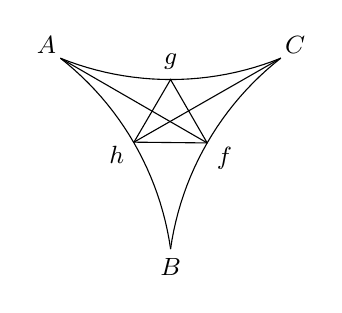
\begin{tikzpicture}[scale=1.4]
				\draw [shift={(-1.651,-2.108)}]  plot[domain=0.141:0.906,variable=\t]({1.*2.678*cos(\t r)+0.*2.677*sin(\t r)},{0.*2.678*cos(\t r)+1.*2.678*sin(\t r)});
				\draw [shift={(1,2.484)}]  plot[domain=4.330:5.095,variable=\t]({1.*2.678*cos(\t r)+0.*2.678*sin(\t r)},{0.*2.678*cos(\t r)+1.*2.678*sin(\t r)});
				\draw [shift={(3.651,-2.108)}]  plot[domain=2.235:3.001,variable=\t]({1.*2.678*cos(\t r)+0.*2.678*sin(\t r)},{0.*2.678*cos(\t r)+1.*2.678*sin(\t r)});
				\draw (0,0) node [above left, xshift=2pt, yshift=-2pt] {\small $A$};
				\draw (2,0) node [above right, xshift=-2pt, yshift=-2pt] {\small $C$};
				\draw (1,-1.732) node [below] {\small $B$};
				\draw (1,-0.194) -- (1.332,-0.769) -- (0.668,-0.762) -- cycle;
				\draw (0,0) -- (1.332,-0.769);
				\draw (2,0) -- (0.668,-0.762);
				\draw (1,-0.194) node [above] {\small $g$};
				\draw (1.332,-0.769) node [below right, yshift=2pt] {\small $f$};
				\draw (0.668,-0.762) node [below left, yshift=2pt] {\small $h$};
				\end{tikzpicture}}
			\fontfamily{cmr}\selectfont
			\caption{Tab. I. Fig. 3.}
		\end{figure}
		\switchcolumn
		\begin{figure}[h]
			\centering
			\par {
				\fontfamily{jkplvos}\selectfont
				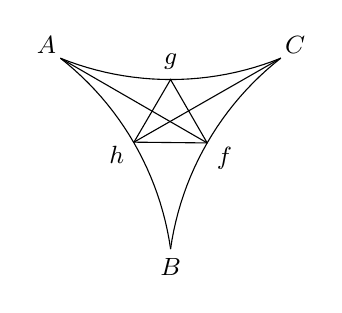
\begin{tikzpicture}[scale=1.4]
				\draw [shift={(-1.651,-2.108)}]  plot[domain=0.141:0.906,variable=\t]({1.*2.678*cos(\t r)+0.*2.677*sin(\t r)},{0.*2.678*cos(\t r)+1.*2.678*sin(\t r)});
				\draw [shift={(1,2.484)}]  plot[domain=4.330:5.095,variable=\t]({1.*2.678*cos(\t r)+0.*2.678*sin(\t r)},{0.*2.678*cos(\t r)+1.*2.678*sin(\t r)});
				\draw [shift={(3.651,-2.108)}]  plot[domain=2.235:3.001,variable=\t]({1.*2.678*cos(\t r)+0.*2.678*sin(\t r)},{0.*2.678*cos(\t r)+1.*2.678*sin(\t r)});
				\draw (0,0) node [above left, xshift=2pt, yshift=-2pt] {\small $A$};
				\draw (2,0) node [above right, xshift=-2pt, yshift=-2pt] {\small $C$};
				\draw (1,-1.732) node [below] {\small $B$};
				\draw (1,-0.194) -- (1.332,-0.769) -- (0.668,-0.762) -- cycle;
				\draw (0,0) -- (1.332,-0.769);
				\draw (2,0) -- (0.668,-0.762);
				\draw (1,-0.194) node [above] {\small $g$};
				\draw (1.332,-0.769) node [below right, yshift=2pt] {\small $f$};
				\draw (0.668,-0.762) node [below left, yshift=2pt] {\small $h$};
				\end{tikzpicture}}
			\fontfamily{cmr}\selectfont
			\caption{Tab. I. Fig. 3.}
		\end{figure}
		
		
		\switchcolumn*
		
		
		
		\item Huiusmodi autem curvas, ex evolutione curvarum triangularium natas, quatenus cum circulo tam egregie conveniunt, brevitatis gratia \textit{Orbiformes} nominemus, hicque ante omnia observasse iuvabit, ex qualibet curva orbiformi problema catoptricum supra memoratum infinitis modus facillime resolvi posse. Sit enim $FGH$ talis curva orbiformes quaecunque, intra qua punctum lucidum $X$ pro lubitu constituatur; tum ducta recta quacunque $Xx$, ad curvam utrinque normali, quae ergo constantem habebit magnitudinem, iungantur rectae $LX$ et $Lx$, eaeque bisecentur in punctis $O$ et $o$, unde ad eas normaliter educantur rectae $OZ$ et $oz$, rectae $Xx$ occurentes in punctis $Z$ et $z$; haecque duo puncta sita erunt in curva quaesita. Radius enim $LZ$, primu reflexus, fiet $Zz$, qui, denuo reflexus in $z$, in ipsum punctum lucidum $L$ remittetur, quemadmodum ex natura reflexionis haud difficulter demonstrare liceret, nisi hoc argumentatum iam uberrime esset pertractatum.
		
		\switchenum
		\item De krommen van deze aard, geboren als evolventen uit driehoekige krommen, voor zover ze uitzonderlijk met een cirkel kunnen overeenkomen, zal ik voor het gemak \textit{Orbiformen} noemen, \textbf{en al deze voorgaande observaties  kunnen helpen}, uit elke orbiforme kromme het voorgaande genoemde \textit{catoptrische} probleem op een oneindig aantal manieren opgelost worden. Als $FGH$ zo'n orbiform is, en hierbinnen uit een punt {\color{red}$L$} gewenste lichtstralen gevormd worden; dan heeft elke rechte $Xx$, langs beide kanten normaal aan de kromme, eenzelfde constante lengte, de rechten $LX$ en $Lx$ worden verbonden, en ze moeten middendoor verdeeld worden in de punten $O$ en $o$, en breng er de normale lijnen $OZ$ en $oz$ aan, rechten die $Xx$ in de punten $Z$ en $z$ ontmoeten; zodat twee punten van de gezochte kromme\footnote{catoprische kromme} \textbf{bekomen} worden. Voor een straal $LZ$, eenmaal weerkaatst, wordt $Zz$, die,  opnieuw weerkaatst in $z$, in hetzelfde punt $L$ wordt teruggebracht, deze manier is uit de aard van terugkaatsing niet moeilijk aan te tonen, \textbf{maar dit argument werd al overvloedig aangeraakt.}
		\switchcolumn*
		
		\begin{figure}[h]
			\centering
			\par {
				\fontfamily{jkplvos}\selectfont
				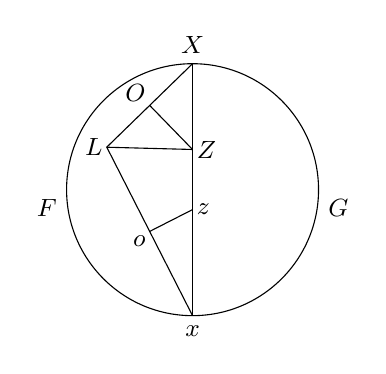
\begin{tikzpicture}[scale=0.8]
				\draw (0,0) circle (2cm);
				\draw (0,-2)-- (0,2);
				\draw (0,-2) -- (-1.362,0.675)-- (0,2);
				\draw (0,0.638)-- (-1.361,0.674);
				\draw (0,0.638)-- (-0.680,1.337);
				\draw (-0.681,-0.663)-- (0,-0.316);
				\draw (0,2) node [above] {\small $X$};
				\draw (0,-2) node [below] {\small $x$};
				\draw (-1.362,0.674) node [left, xshift=2pt] {\small $L$};
				\draw (-0.680,-0.662) node [below left, xshift=2pt, yshift=2pt] {\small $o$};
				\draw (-0.680,1.337) node [above left, xshift=2pt, yshift=-2pt] {\small $O$};
				\draw (0,0.637) node [right, xshift=-2pt] {\small $Z$};
				\draw (0,-0.316) node [right, xshift=-2pt] {\small $z$};
				\draw (-2.,0.) node [below left] {\small $F$};
				\draw (2.,0.) node [below right] {\small $G$};
				\end{tikzpicture}}
			\fontfamily{cmr}\selectfont
			\caption{Tab. I. Fig. 4.}
		\end{figure}
		\switchcolumn
		\begin{figure}[h]
			\centering
			\par {
				\fontfamily{jkplvos}\selectfont
				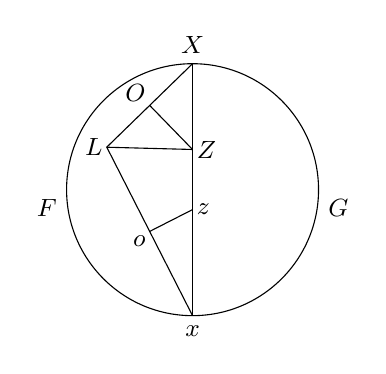
\begin{tikzpicture}[scale=0.8]
				\draw (0,0) circle (2cm);
				\draw (0,-2)-- (0,2);
				\draw (0,-2) -- (-1.362,0.675)-- (0,2);
				\draw (0,0.638)-- (-1.361,0.674);
				\draw (0,0.638)-- (-0.680,1.337);
				\draw (-0.681,-0.663)-- (0,-0.316);
				\draw (0,2) node [above] {\small $X$};
				\draw (0,-2) node [below] {\small $x$};
				\draw (-1.362,0.674) node [left, xshift=2pt] {\small $L$};
				\draw (-0.680,-0.662) node [below left, xshift=2pt, yshift=2pt] {\small $o$};
				\draw (-0.680,1.337) node [above left, xshift=2pt, yshift=-2pt] {\small $O$};
				\draw (0,0.637) node [right, xshift=-2pt] {\small $Z$};
				\draw (0,-0.316) node [right, xshift=-2pt] {\small $z$};
				\draw (-2.,0.) node [below left] {\small $F$};
				\draw (2.,0.) node [below right] {\small $G$};
				\end{tikzpicture}}
			\fontfamily{cmr}\selectfont
			\caption{Tab. I. Fig. 4.}
		\end{figure}

		\switchcolumn*

		\item Ob hunc insignem usum curvarum triangularium utique optandum esset, ut methodus certa pateret, cuius ope huismodi curvas triangulares, quotquot libuerit, investigare liceret, id quod primo intuitu nimis difficile videre potest. Verum hunc investigationem invertamus, ac primo quaeramus curvas orbiformes, quales hactenus descripsimus; tum enim certi esse poterimus, earum evolutas huismodi fore curvas triangular quales desideramus, Praeterea vero etiam hoc modo istud commodum assequemur: ut, quoties curva orbiformis fuerit algebraica, toties quoque curva triangularis non solum fiat algebraica, sed insuper etiam rectificabilis, quandoquidem evolutae omnium curvarum algebraicarum simul rectificationem admittunt.
		
		\switchenum
		\item Door het buitengewone gebruik van driehoekige krommen, zou het zonder twijfel wenselijk zijn, om bepaalde methodes te bereiken die het mogelijk maken deze driehoekige krommen, zoveel je wil, mogelijk te te bepalen, wat op het eerste zicht zeer moeilijk in te zien is. Maar het onderzoek wordt omgedraaid, waar ten eerste de orbiforme krommen gezocht worden,  zoals tot dusver beschreven, \textbf{want dan zijn we zeker dat we in staat zijn, hun ontwikkeling van de soort driehoekige krommen zal zijn zoals we wensen, bovendien is dit op deze manier handig te bereiken}: zo wanneer de orbiforme kromme algebraïsch is, is ook de driehoekige kromme niet enkel algebraïsch, maar bovendien ook te herleiden, aangezien de ontwikkeling van alle algebraïsche krommen ook een herleiding toelaten.
		
		\switchcolumn*
		
		\item Sit igitur $FMfm$ talis curva orbiformis, qualem investigare nobis est propositum, in qua sumamus rectam $Ff$ pro axe fixo, qui utrinque ad curvam sit normalis cuius longitudinem ponamus $Ff=2f$. Tum ex puncto quocunque $M$ ad curvam ducatur normalis $Mm$ quae ergo etiam in $m$ ad curvam debet esse normalis, eiusque longitudo $Mm$ itidem sit $=2f$. Iam ex punctis $M$ et $m$ ad axem $Ff$ demittantur perpendicula $Pm$ et $pm$, ac pro puncto $M$ vocentur coordinatae $FP=X$ et $PM=Y$; at pro puncto $m$ sit $Fp=x$ et $pm = -y$, quia haec applicata in partem contrariam cadit. His positis talis aequatio inter $X$ et $Y$ desideratur, ut, si loco $X$ scribatur $x$, valor ipsius $Y$ sponte prodeat $=-y$. 
		
		\switchenum
		\item Laat $FMfm$ een orbiforme kromme zijn, wat ons is voorgesteld te onderzoeken, waardoor we een rechte lijn $Ff$ drijven, die normaal is aan de kromme aan beide zijden, waarvan we de lengte $Ff=2f$ noemen. Dan voor elk ander punt $M$ wordt de normaal aan de kromme getekend zodat deze ook in $m$ normaal is aan de kromme, en deze lengte $Mm$ is ook $=2f$. Door de punten $M$ en $m$ wordt op de as $Ff$ de loodrechten $PM$ en $pm$ getekend, en noem de coördinaten van het punt $M$ via $FP=XF$ en $PM=Y$; in het punt $m$ is $Fp=x$ en $pm=-y$, dit is toegepast in tegengestelde richting. Zo'n vergelijking tussen de plaatsen $X$ en $Y$ is gewenst, zo, als de plaats $X$ als $x$ geschreven wordt, voor de waarde van $Y$ spontaan verschijnt $=-y$. \textbf{ Maar om dit te laten gebeuren, zou de gehele kromme $FMfm$ niet doorlopend zijn.} 
		
		\switchcolumn*
		
		\begin{figure}[h]
			\centering
			\par {
				\fontfamily{jkplvos}\selectfont
				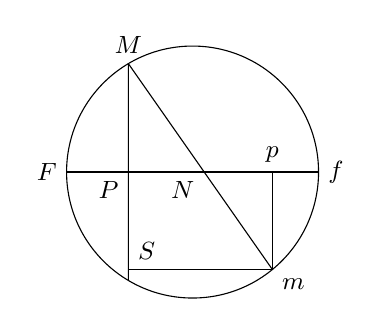
\begin{tikzpicture}[scale=0.8]
				\draw (0,0) circle (2cm);
				\draw (-2,0)-- (2,0);
				\draw (-1.019,1.721)-- (1.267,-1.547);
				\draw (-1.019,1.721)-- (-1.020,-1.720);
				\draw (-1.019,-1.547)-- (1.267,-1.547);
				\draw (1.267,-1.547)-- (1.267,0.);
				\draw (-1.0192,1.720) node [above] {\small $M$};
				\draw (-2.,0.) node [left] {\small $F$};
				\draw (2.,0.) node [right] {\small $f$};
				\draw (-1.0193,0.) node [below left] {\small $P$};
				%\draw (-1.0193,-1.721) node [above] {\small $e$};
				\draw (1.267,-1.547) node [below right] {\small $m$};
				\draw (0.184,0.) node [below left] {\small $N$};
				\draw (1.267,0.) node [above] {\small $p$};
				\draw (-1.019,-1.547) node [above right] {\small $S$};
				\end{tikzpicture}}
			\fontfamily{cmr}\selectfont
			\caption{Tab. I. Fig. 5.}
		\end{figure}
		\switchcolumn
		\begin{figure}[h]
			\centering
			\par {
				\fontfamily{jkplvos}\selectfont
				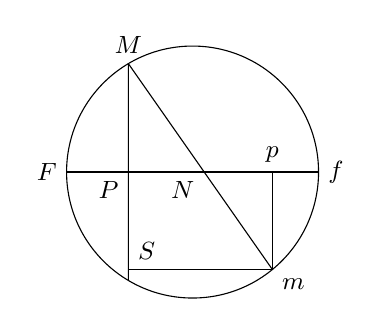
\begin{tikzpicture}[scale=0.8]
				\draw (0,0) circle (2cm);
				\draw (-2,0)-- (2,0);
				\draw (-1.019,1.721)-- (1.267,-1.547);
				\draw (-1.019,1.721)-- (-1.020,-1.720);
				\draw (-1.019,-1.547)-- (1.267,-1.547);
				\draw (1.267,-1.547)-- (1.267,0.);
				\draw (-1.0192,1.720) node [above] {\small $M$};
				\draw (-2.,0.) node [left] {\small $F$};
				\draw (2.,0.) node [right] {\small $f$};
				\draw (-1.0193,0.) node [below left] {\small $P$};
				%\draw (-1.0193,-1.721) node [above] {\small $e$};
				\draw (1.267,-1.547) node [below right] {\small $m$};
				\draw (0.184,0.) node [below left] {\small $N$};
				\draw (1.267,0.) node [above] {\small $p$};
				\draw (-1.019,-1.547) node [above right] {\small $S$};
				\end{tikzpicture}}
			\fontfamily{cmr}\selectfont
			\caption{Tab. I. Fig. 5.}
		\end{figure}
		
		\switchcolumn*
		
		\par Nisi enim hoc fieret, tota curva $FMfm$ non esset continua. Sequenti autem modo hae quatuor quantitates a se inuicem pendent: Cum intervallum $PN$ sit subnormalis respectu puncti $M$, posito $\D Y = P \,\D X$, erit haec subnormalis $PN=PY$, hincque normalis $MN=Y\sqrt{1+PP}$. Simili modo  altero puncto $m$ erit $pN$ subnormalis retro posita; unde sumto $\D y=p\,\D x$ erit $pN = -py$; hinc normalis $mN = -y\sqrt{1+pp}$. Quia igitur triangula $PMN$ et $pmN$ sunt similia, erit $P=p$. 
		
		\newpage
		
		Porro quia nuimus esse $Mm=2f$; ex $m$ agatur axi parallela $mS$, ipsi $MP$ productae occurens in $S$, et similitudo triangulorum $MNP$ et $MmS$ dabit $MS = \frac{2f}{\sqrt{1+pp}}$ et $mS = \frac{2fp}{\sqrt{1+pp}}$.
		\par Cum igitur fit
		\[
			MS = MP + mp = Y-y  \quad \text{et} \quad mS = Fp-FP = x-X
		\]
		hinc colligitur
		\[
			Y-y = \frac{2f}{\sqrt{1+pp}} \quad \text{et}\quad x-X = \frac{2fp}{\sqrt{1+pp}},
		\]
		
		\par praeterea vero, uti iam notauimus, debet esse
		\[
			\frac{\D Y}{\D X} = P = p \quad \text{et} \quad \frac{\D y}{\D x} = p.
		\]
		
		\switchcolumn
		
		\par Er volgt de manier waarop deze vier eenheden met elkaar in verband staan: Omdat de afstand van het punt $M$ tot $PN$ subnormaal is, is positie $\D Y = P \,\D X$ , hieruit volgt voor de subnormaal\footnote{Verwarrend van Euler dat het maal-teken niet genoteerd wordt en hier dus een product van scalair en afstand rechts staat.} $PN = P\cdot Y$,  vandaar de normaal $MN = Y\sqrt{1+PP}$. Op gelijkaardige manier zal voor het andere punt $m$ de subnormaal $pN$ terug bepaald zijn; neemt men $\D y = p \, \D x$, dan\footnote{Dezelfde verwarring neemt hier plaats.} $pN=-p\cdot y$; hierdoor geldt voor de normaal $Mn=-y\sqrt{1+pp}$. Omdat de driehoeken $PMN$ en $pmN$ gelijkvormig zijn, geldt $P=p$. 
		
		\newpage
		Omdat we verder weten dat $Mm=2f$; maak uit $m$ evenwijdig aan de as, \textbf{$MP$ zichzelf verlengend onmoeten in $S$}, en de gelijkvormige driehoeken $MNP$ en $MmS$ leiden tot $MS = \frac{2f}{\sqrt{1+pp}}$ et $mS = \frac{2fp}{\sqrt{1+pp}}$.
		\par Aangezien derhalve het wordt dat
		\[
			MS = MP + mp = Y-y  \quad \text{en} \quad mS = Fp-FP = x-X
		\]
		hieruit volgt
		\[
			Y-y = \frac{2f}{\sqrt{1+pp}} \quad \text{en}\quad x-X = \frac{2fp}{\sqrt{1+pp}},
		\]
		\par daarnaast echter, zoals we al hebben opgemerkt, moet het zijn dat
		\[
			\frac{\D Y}{\D X} = P = p \quad \text{en} \quad \frac{\D y}{\D x} = p.
		\]
				
		\switchcolumn*
		
		\item Cum igitur inuenerimus differentias coordinatarum $Y-y$ et $x-X$, statuamus earum summas $X+x= 2Q$ et $Y+y=2R$, hincque singulas coordinatas adipiscemur ita expressas:
		\begin{align*}
			X &= Q - \frac{fp}{\sqrt{1+pp}}; \quad Y = R + \frac{f}{\sqrt{1+pp}};\\
			x &= Q+\frac{fp}{\sqrt{1+pp}}; \quad y= R- \frac{f}{\sqrt{1+pp}}.
		\end{align*}
		\par Hinc igitur differentiando erit
		\begin{align*}
			\D X &= \D Q - \frac{f\,\D p}{(1+pp)^\frac{3}{2}};\\
			\D Y &= \D R-\frac{fp\,\D p}{(1+pp)^\frac{3}{2}};\\
			\D x &= \D Q + \frac{f\,\D p}{(1+pp)^\frac{3}{2}};\\
			\D y &= \D R + \frac{fp\,\D p}{(1+pp)^\frac{3}{2}}.\\
		\end{align*}
		\par Cum igitur esse debeat $\D Y=p\,\D X$ et $\D y=p\,\D x$, fiet
		\begin{align*}
			\D R - \frac{fp\,\D p}{(1+pp)^\frac{3}{2}} &= p\operatorname{d}Q - \frac{fp\, \D p}{(1+pp)^\frac{3}{2}} \quad \text{et}\\
			\D R + \frac{fp\,\D p}{(1+pp)^\frac{3}{2}} &= p\,\D Q + \frac{fp\,\D p}{(1+pp)^\frac{3}{2}}.
	 	\end{align*}
	 	
		\par Ex utraque harum aequationum sequitur fore $\operatorname{d} R = p\,\D  Q$, ideoque $R = \int p \,\D Q$.
		
		\switchenum
		\item We vinden zo als verschil van coördinaten $Y-y$ en $x-X$, waarvan we de sommen $X+x=2Q$ en $Y+y=2R$ vastleggen, er volgt dat de enkele coördinaten uitgedrukt kunnen worden als:
		\begin{align*}
			X &= Q - \frac{fp}{\sqrt{1+pp}}; \quad Y = R + \frac{f}{\sqrt{1+pp}};\\
			x &= Q+\frac{fp}{\sqrt{1+pp}}; \quad y= R- \frac{f}{\sqrt{1+pp}}.
		\end{align*}
		\par Dit afleiden leidt tot:
		\begin{align*}
			\D X &= \D Q - \frac{f\,\D p}{(1+pp)^\frac{3}{2}};\\
			\D Y &= \D R-\frac{fp\,\D p}{(1+pp)^\frac{3}{2}};\\
			\D x &= \D Q + \frac{f\,\D p}{(1+pp)^\frac{3}{2}};\\
			\D y &= \D R + \frac{fp\,\D p}{(1+pp)^\frac{3}{2}}.\\
		\end{align*}
		\par Waarbij het zo moet zijn dat $\D Y=p\,\D X$ et $\D y=p\,\D x$, wat wordt
		\begin{align*}
			\D R - \frac{fp\,\D p}{(1+pp)^\frac{3}{2}} &= p\operatorname{d}Q - \frac{fp\, \D p}{(1+pp)^\frac{3}{2}} \quad \text{en}\\
			\D R + \frac{fp\,\D p}{(1+pp)^\frac{3}{2}} &= p\,\D Q + \frac{fp\,\D p}{(1+pp)^\frac{3}{2}}.
		\end{align*}
		\par Uit beide van deze vergelijkingen volgt $\D R = p \, \D Q$, zodat $R= \int p \,\D Q$.
		\switchcolumn*
		
		\item Cum igitur omnibus conditionibus satisfecerimus, quantitas $Q$ arbitrio nostro permittitur, eiusque ergo loco functio quaecunque ipsius $p$ accipi poterit, quae autem ita debet esse comparata, ut formula $p\,\D Q$ integrationem admittat, siquidem curvas algebraicas desideremus. Quoniam igitur pro coordinatis $x$ et $y$ invenimus:
		\[
			x = Q + \frac{fp}{\sqrt{1+pp}} \quad\text{et}\quad y = R - \frac{f}{\sqrt{1+pp}}
		\]
		\par existente $R = \int p \,\D Q$; pro alteris vero coordinatis $X$ et $Y$ sit
		\[
			X = Q- \frac{fp}{\sqrt{1+pp}} \quad \text{et} \quad Y = R + \frac{f}{\sqrt{1+pp}},
		\]
		manifestum est, has ex illis nasci, si modo formulae radicalis $\sqrt{1+pp}$ signum immutetur. Quare cum haec formula per suam naturam sit ambigua, priores formulae, pro $x$ et $y$ inventae, posteriores pro $X$ et $Y$ iam sponte involuunt, ita ut eadem aequatio rationalis tam pro $x$ et $y$ quam pro $X$ et $Y$ necessario sit proditura. Ad hoc autem necesse est, ut neque $Q$ neque $R$ eandem formulam $\sqrt{1+pp}$ involuant, quia alioquin etiam signum harum litterarum mutari oporteret. Hinc igitur ista regula statui potest: ut pro $Q$ functio rationalis ipsius $p$ accipi debeat.
		
		\switchenum
		\item Als ik derhalve voldoe aan alle voorwaarden, laat dit ons een keuze van hoeveelheid $Q$ toe, en kan daarom in de plaats wat dan ook van functie van $p$ aanvaarden, als het toegelaten is de formule $p\,\D Q$ te integreren, omdat we een algebraïsche kromme wensen. Zo vinden we voor de coördinaten $x$ en $y$:
		\[
			x = Q + \frac{fp}{\sqrt{1+pp}} \quad\text{et}\quad y = R - \frac{f}{\sqrt{1+pp}}
		\]
		als $R=\int p \,\D Q$ bestaat; voor zeker zijn de andere coördinaten duidelijk
		\[
			X = Q- \frac{fp}{\sqrt{1+pp}} \quad \text{et} \quad Y = R + \frac{f}{\sqrt{1+pp}},		
		\]
		
		\newpage
		
		wat geboren is uit het vorige, waarbij enkel het teken van de wortelvorm $\sqrt{1+pp}$ gewijzigd is. Waarom is deze formule van nature onzeker\footnote{Niet vast bepaald? Inwisselbaar?}, eerste formules, voor $x$ en $y$ die gevonden zijn, impliceren spontaan de volgende voor $X$ en $Y$,zodat dezelfde rationale vergelijkingen zo voor $x$ en $y$, als voor $X$ en $Y$ niet noodzakelijk wordt gemaakt. Hiervoor is het meer bepaald noodzakelijk dat noch $Q$ noch $R$ dezelfde formule $\sqrt{1+pp}$ \textbf{betrekken}, want anders wordt ook het teken van deze letter gewijzigd.  Voor deze reden is het een regel die voorgeschreven mag worden: zo moet voor $Q$ een rationale functie van $p$ aanvaard worden.
		
		
		\switchcolumn*
		
		\item Ut autem curvas algebraicas obtineamus, quia esse debet $R = \int p \,\D Q = pQ - \int Q \,\D p$; statuamus $\int Q \,\D p = S$, denotante $S$ functionem quamcunque rationalem ipsius $p$, eritque $Q = \frac{\D S}{\D p}$, hincque porro $R = \frac{p\,\D S}{\D p}-S$. Nunc igitur pro curvis orbiformibus sequentes determinationes ambarum coordinatarum $x$ et $y$ exhibere possumus:
		\[
			x = \frac{\D S}{\D p} + \frac{fp}{\sqrt{1+pp}}, \quad y = \frac{p\,\D S}{\D p} -S - \frac{f}{\sqrt{1+pp}},
		\]
		ubi pro $S$ functionem quamcunque rationalem ipsius $p$, vel saltem talem, accipere possumus, quae, dum formula $\sqrt{1+pp}$ est ambigua, eundem valorem retineat.
		
		\switchenum
		\item Om een algebraïsche kromme te verkrijgen, moet het zijn dat $R = \int p \,\D Q = pQ - \int Q \,\D p$; we krijgen  $\int Q \,\D p = S$, stel met $S$ een zekere rationale functie voor van $p$, en dan $Q = \frac{\D S}{\D p}$, vandaar verder $R = \frac{p\,\D S}{\D p}-S$. En dus vervolgens voor de orbiforme kromme kunnen we aantonen dat beide coördinaten $x$ en $y$ verkregen worden door: 
		\[
			x = \frac{\D S}{\D p} + \frac{fp}{\sqrt{1+pp}}, \quad y = \frac{p\,\D S}{\D p} -S - \frac{f}{\sqrt{1+pp}};
		\]
		\textbf{wanneer we voor $S$ sommige rationale functies van $p$, of minstens zodanig, kunnen nemen, wat hoewel de formule $\sqrt{1+pp}$ onbepaald is, dezelfde waarde behoudt.}
		
		\switchcolumn*
		
		\item Quia natura orbis, qualem consideramus, postulat, ut curva sit in se rediens, et nusquam in infinitum porrigatur, functio $S$ ita comparata esse debet, ut neque absicissa $x$ neque applicata $y$ unquam fieri possit infinita, quem in finem hanc functionem $S$ tali fractioni:
		\[
			\frac{\alpha+\beta}{A+B}\frac{p+\gamma }{p+C} \frac{p p+\delta}{p p+D} \frac{p^3+\text{etc}.}{p^3+\text{etc}.}
		\]
		\par aequari opportet, cuius denominator nullum habeat factorem simplicem realem; si enim factorem talem haberet puta $p-n$, tum, sumto $p=n$, valor ipsius $S$ fieret infinitus. Deinde summa potestas ipsius $p$ in numeratore haud debet esse major quam in denominatore; aliter enim, casu $p=\infty$, alor ipsius $S$ iterum in infinitum excresceret.
		
		\newpage
		
		Praeterea vero etiam exponentes fracti ipsius $p$ admitti quidem possent, ita tamen, ut nullum membrum ambiguum obtineat valorem, quia alioquin eidem valori ipsius $p$ plures tam abscissae quam applicatae convenire possent; hoc enim casu curva non post unam revolutionem, sed demum post duas pluresue in se rediret; tum autem eius evoluta non amplius foret curva triangularis, sed vel pentagona, vel heptagona, vel enneagona vel etc. id quod insituto nostro adversatur.
		
		\switchenum
		\item Het is vereist wegens het essentie de cirkel, hetgeen we beschouwen, als de kromme in zichzelf terugkeert, en zich nooit oneindig verspreid\footnote{Met andere woorden, de kromme moet zich opnieuw bij zichzelf aansluiten als bij een cirkel.}, de functie $S$ die moet worden voorbereid, dat noch de absis $x$ noch de ordinaat $y$ ooit in staat zijn oneindig te worden, \textbf{om uiteindelijk de functie $S$ op te breken als:}
		\[
			\frac{\alpha+\beta}{A+B}\frac{p+\gamma }{p+C} \frac{p p+\delta}{p p+D} \frac{p^3+\text{etc}.}{p^3+\text{etc}.}
		\]
		\par het is evengoed nodig dat, als de noemer nul bevat de factoren reëel vereenvoudigen; als er zo'n factor bevat is, bijvoorbeeld $p-n$, dan, in het geval dat $p=n$, zal de waarde van $S$ oneindig worden. Vandaar de macht van $p$ in de teller groter moet zijn dan in de noemer; anderzijds, in het geval dat $p=\infty$, dan zal de waarde van $S$ opnieuw naar oneindig groeien.
		
		\newpage
		
		Meer bepaald kunnen ook breuken als exponent van $p$ toegelaten worden, zodanig dat, er geen onbepaalde delen als waarde bekomen worden, daarnaast is zelfs het mogelijk dat voor meerdere waarden van $p$ zo de abscis als ordinaat samen komen; maar in dit geval zal de kromme uiteindelijk niet na één onwenteling, maar na twee of meer in zichzelf terugkomen;  dan meer bepaal zal zijn evolute niet meer de driehoekige kromme, maar wel de vijfhoekige, of zevenhoekige, of negenhoekige of etc. wat tegen onze opzet is.
		

		\switchcolumn*
		
		\item Ex hac constructione generali, in qua continentur omnes curvae orbiformes, et quidem simplices, quae post unam ontwikkeling in se redeunt, facile erit formulas elicere pro descriptione curvarum triangularium; cum enim evolutae harum curvarum orbiformium certe sint figurae triangulares, tantum opus est, ut in evolutas istarum curvarum inquiramus. Quia autem omnes illae curvae, pro quovis valore litterae $f$, ex evolutione eiusdem curvae triangularis nascuntur, littera $f$ non in determinationem evolutae ingreditur; unde in formulis nostris, pro $x$ et $y$ inventis, partes, hanc litteram $f$ involventes, tuto omittere licebit; sicque pro hac inventigatione habebimus tantum
		\[
			x = \frac{\D S}{\D P} \quad\text{et} \quad y = \frac{p\,\D S}{\D p}-S,
		\]
		\par quam ob rem naturam evolutae, ex his valoribus oriundae, investigasse sufficiet. 
		
		\switchenum
		\item Uit dit volgt een algemene constructie, waarin alle orbiforme krommen bevat zitten, en dit vereenvoudigt, na een revolutie om zichzelf, gemakkelijk in formules die driehoekige krommen beschrijven. Want met de evolute van deze orbiforme kromme zijn er zeker driehoekige figuren, alleen is het noodzakelijk, dat we moeten zoeken naar de evoluten van deze kromme. Omdat al die krommen, voor elke waarde van de letter $f$, uit de evolvente van eenzelfde driehoekige kromme geboren zijn, is de letter $f$ niet bepalend in de evolute bevat; en in onze formule, voor de gevonden $x$ en $y$, is het toegestaan de delen , die de letter $f$ bevatten, geheel weg te laten; en dus hebben we voor dit onderzoek alleen
		\[
			x = \frac{\D S}{\D P} \quad\text{et} \quad y = \frac{p\,\D S}{\D p}-S,
		\]
		wat voldoende is om de zaak van de natuurlijke evolute, uit deze waarden voortkomend, te onderzoeken.
		
		\switchcolumn*
		
		\item Sit igitur $FMfm$ talis curvas, in qua sit abscissa $FP=x=\frac{\D S}{\D p}$, applicata $PM=y=\frac{p\,\D }{\D p}-S$, et ducta normali $Mm$ erit subnormalis
		\[
			PN = py = \frac{pp\,\D S}{\D p}-pS
		\]
		unde sit recta
		\[
			FN = \frac{\D S}{\D p}(1+pp)-pS.
		\]
		\par Ponamus nunc angulum $FNM = \phi$, erit $\tang \phi = \frac{1}{p}$, ideoque $p=\cotg \phi = \frac{\cosg \phi}{\sing \phi}$, unde fit
		\[
			\sing \phi = \frac{1}{\sqrt{1+pp}} \quad \text{et} \quad \cosg \phi = \frac{p}{\sqrt{1+pp}}
		\]
		tum vero etiam $\D \phi = -\frac{\D p}{1+pp}$. Quod si iam brevitatis gratia ponamus $FN=v$, notum est, centrum circuli, curvam in $M$ osculantis, fore in puncto $U$, ita ut sit
		\[
			NU = \frac{\D v\sing \phi}{\D \phi};
		\]
		Cum autem, sumto elemento $\D p$ constante, sit
		\begin{align*}
			\D  v &= \frac{\D \D  S}{\D p}(1+pp)+p\,\D S-S\,\D p \quad \text{et}\\
			\frac{\sing \phi}{\D \phi} &= -\frac{\sqrt{1+pp}}{\D p}
		\end{align*}
		erit recta
		\[
			NU = -\frac{\D\D S}{\D p^2} (1+pp)^{\frac{3}{2}}-\frac{p\,\D S}{\D p} \sqrt{1+pp} + S\sqrt{1+pp}
		\]
		\par pro qua formula brevitatis ergo scribamus $r$, ita ut vit sit $NU=r$.
		
		\switchenum
		\item Laat nu $FMfm$ een dergelijke curve zijn, waarin de abscis $FP=x=\frac{\D S}{\D p}$, benoem $PM=y=\frac{p\, \D S}{\D p}-S$, en uit de normaal $Mn$ ontstaat de subnormaal
		\[
			PN = py = \frac{pp\,\D S}{\D p}-pS
		\]
		\par zodat de lijn
		\[
			FN = \frac{\D S}{\D p}(1+pp)-pS.
		\]
		\par Benoem nu de hoek $FNM = \phi$, zodat $\tang \phi = \frac{1}{p}$, zodat $p = \cotg \phi = \frac{\cosg \phi}{\sing \phi}$, en dit resulteert in
		\[
			\sing \phi = \frac{1}{\sqrt{1+pp}} \quad \text{et} \quad \cosg \phi = \frac{p}{\sqrt{1+pp}}
		\]
		\par dan geldt ook $\D \phi = -\frac{\D p}{1+pp}$. Stel nu voor het gemak de afkorting $FN=v$, het is geweten dat het centrum van de osculatiecirkel in $M$, in het punt $U$ is, dan is het zo\footnote{Waar komt dit vandaan?}
		\[
			NU = \frac{\D v\sing \phi}{\D \phi};
		\]
		\par Maar als, het element $\D p$ constant genomen wordt, is
		\begin{align*}
			\D  v &= \frac{\D \D  S}{\D p}(1+pp)+p\,\D S-S\,\D p \quad \text{en}\\
			\frac{\sing \phi}{\D \phi} &= -\frac{\sqrt{1+pp}}{\D p}
		\end{align*}
		\par en de lijn zal zijn
		\[
			NU = -\frac{\D\D S}{\D p^2} (1+pp)^{\frac{3}{2}}-\frac{p\,\D S}{\D p} \sqrt{1+pp} + S\sqrt{1+pp}
		\]
		\par voor het gemak van afkorting schrijven we voor de formule $r$, zodat er geldt $NU=r$.

		\switchcolumn*
		
		\begin{figure}[h]
			\centering
			\par {
				\fontfamily{jkplvos}\selectfont
				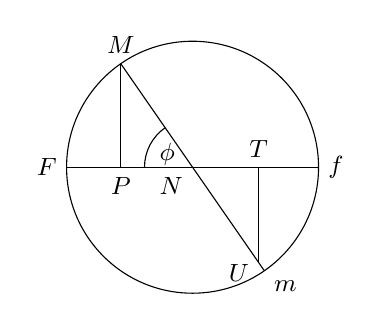
\begin{tikzpicture}[scale=0.8]
				\draw (124.73955121402813:0.7631107015839075) arc (124.73955121402813:180.:0.7631107015839075);
				\draw (0,0) circle (2cm);
				\draw (-1.1396938257701044,1.643501744295242)-- (1.1396938257701044,-1.643501744295242);
				\draw (1.0499141426476895,-1.5140344588914103)-- (1.0499141426476895,0.);
				\draw (-1.1396938257701044,0.)-- (-1.1396938257701044,1.643501744295242);
				\draw (-2,0)-- (2,0);
				
				\draw (0,0) node [below left] {\small $N$};
				\draw (-2,0) node [left] {\small $F$};
				\draw (2,0) node [right] {\small $f$};
				\draw (-1.1396938257701044,1.643501744295242) node [above] {\small $M$};
				\draw (1.1396938257701044,-1.643501744295242) node [below right] {\small $m$};
				\draw (-1.1396938257701044,0.) node [below] {\small $P$};
				\draw (1.0499141426476895,-1.5140344588914103) node [below left,yshift=3pt] {\small $U$};
				\draw (1.0499141426476895,0.) node [above] {\small $T$};
				\draw (-0.4,0.2) node {\small $\phi$};
				\end{tikzpicture}}
			\fontfamily{cmr}\selectfont
			\caption{Tab. I. Fig. 6.}
		\end{figure}
		\switchcolumn
		\begin{figure}[h]
			\centering
			\par {
				\fontfamily{jkplvos}\selectfont
				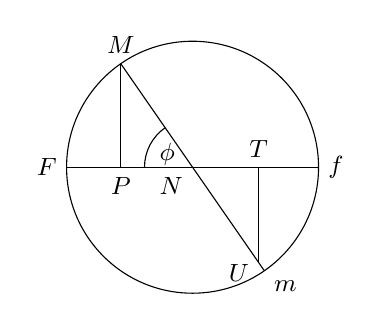
\begin{tikzpicture}[scale=0.8]
				\draw (124.73955121402813:0.7631107015839075) arc (124.73955121402813:180.:0.7631107015839075);
				\draw (0,0) circle (2cm);
				\draw (-1.1396938257701044,1.643501744295242)-- (1.1396938257701044,-1.643501744295242);
				\draw (1.0499141426476895,-1.5140344588914103)-- (1.0499141426476895,0.);
				\draw (-1.1396938257701044,0.)-- (-1.1396938257701044,1.643501744295242);
				\draw (-2,0)-- (2,0);
				
				\draw (0,0) node [below left] {\small $N$};
				\draw (-2,0) node [left] {\small $F$};
				\draw (2,0) node [right] {\small $f$};
				\draw (-1.1396938257701044,1.643501744295242) node [above] {\small $M$};
				\draw (1.1396938257701044,-1.643501744295242) node [below right] {\small $m$};
				\draw (-1.1396938257701044,0.) node [below] {\small $P$};
				\draw (1.0499141426476895,-1.5140344588914103) node [below left,yshift=3pt] {\small $U$};
				\draw (1.0499141426476895,0.) node [above] {\small $T$};
				\draw (-0.4,0.2) node {\small $\phi$};
				\end{tikzpicture}}
			\fontfamily{cmr}\selectfont
			\caption{Tab. I. Fig. 6.}
		\end{figure}

		\switchcolumn*
		\newpage
		
		\item Invento puncto $U$, quod erit in evoluta quam quaerimus, inde axem ducamus perpendiculum $UT$, ac pro evoluta vocemus abscissam $FT=t$ et applicatam $TU=u$; erit autem:
		\begin{align*}
			NT &= NU \cosg \phi = \frac{pr}{\sqrt{1+pp}} \quad \text{et}\\
			TU &= NU \sing \phi = \frac{r}{\sqrt{1+pp}}
		\end{align*}
		unde, loco r valorem assumtum substitutuendo, consequemur abscissam
		\[
			t = FN + NT = \frac{\D S}{\D p} - \frac{p\,\D\D S}{\D p^2} (1+pp),
		\]
		tum vero applicatam
		\[
			u = S - \frac{p\, \D S}{\D p}-\frac{\D \D S}{\D p^2}(1+pp);
		\]
		unde colligimus
		\[
			t-pu = \frac{\D S}{\D p}(1+pp)-pS.
		\]
		\par Ope igitur harum formularum, quaecunque functio idonea ipsius $p$ pro $S$ accipiatur, tam abscissam $FT = t$ quam applicatam $TU=u$ assignare poterimus, quibus curva triangularis determinatur. Valores autem idoneas, pro $S$ accipiendos, supra indicauimus.
		
		\switchenum
		\newpage
		\item We zijn op zoek naar, het vinden van het punt $U$, wat de evolute zal zijn, daarvoor leiden we een loodlijn $UT$ op de as, en voor de evolute noemen we de abscis $FT=t$ en ordinaat $TU=u$, zodat het is
		\begin{align*}
			NT &= NU \cosg \phi = \frac{pr}{\sqrt{1+pp}} \quad \text{en}\\
			TU &= NU \sing \phi = \frac{r}{\sqrt{1+pp}}
		\end{align*}
		en, substitueer op de plaats van $r$ de gevonden waarde, bereikt de abscis
		\[
			t = FN + NT = \frac{\D S}{\D p} - \frac{p\,\D\D S}{\D p^2} (1+pp),
		\]
		vervolgens de waarde van de ordinaat
		\[
			u = S - \frac{p\, \D S}{\D p}-\frac{\D \D S}{\D p^2}(1+pp);
		\]
		hieruit zien we dat
		\[
			t-pu = \frac{\D S}{\D p}(1+pp)-pS.
		\]
		\par Dus met behulp van deze formules, als een geschikte functie voor $S$ uit $p$ genomen wordt, kunnen we zo de abscis $FT=t$ als de ordinaat $TU=u$ toewijzen, die een driehoekige kromme bepalen. Zolang voor $S$ geschikte waarden aanvaard worden, zoals hierboven aangegeven.
		
		\switchcolumn*
		
		\item Quo hanc investigationem exemplo illustremus, sumamus
		\begin{align*}
			S &= \frac{ap}{1+pp}, \quad\text{eritque}\\
			\frac{\D S}{\D p} &= \frac{a(1-pp)}{(1+pp)^2} \quad \text{et} \quad \frac{\D \D S}{\D p^2} = \frac{2ap^3-6ap}{(1+pp)^3}
		\end{align*}

		unde colligimus
		\[
			t = \frac{a+5app-2ap^4}{(1+pp)^2}\quad \text{et} \quad u = \frac{6ap}{(1+pp)^2}.
		\]
		\par Hinc primo patet, sive $p$ sumatur positve sive negative, abscissam $t$ eandem manere, applicatam vero $u$ hoc casu in partem contrariam cadere, unde noster $FT$ huius curvae erit diameter. Deinde, sumto $p=0$ fiet $t=a$ et $u=0$; at si capiatur $p$ inifite parvum, fiet
		\[
			t = a + 3app\quad \text{et} \quad u= 6ap.
		\]
		\par Porro, sumto $p=\frac{1}{2}$, erit $t=\frac{34}{25}a$ et $u=\frac{48}{25}a$; sin autem $p=1$ erit $t=a$ et $u=\frac{3}{2}a$. Sit denique $p=\infty$, eritque $t=-2a$ et $u=0$. Hinc patet, curvam huismodi figuram esse habituram, qualem in figura ei dedimus, ternas cuspides habentem, $B,C,D$, existente $FD=2a$ et $FA=a$. Pro alteris cuspidibus $B$ et $C$ quaeratur locus, ubi applicata $u$ fit maxima, et cum sit
		\[
			\D.\frac{p}{(1+pp)^2} = \frac{\D p(1-3pp)}{(1+pp)^3}
		\]
		hoc eueniet, ubi $3pp=1$, sive $p=\frac{1}{\sqrt{3}}$; tum autem fiet abscissa $t=\frac{11}{8}a$ et $u=\frac{9\sqrt{3}}{8}a$. Ergo ducta chorda $BC$, axem secante in $E$, erit $FE= \frac{11}{8}a$ et $EB=EC=\frac{9\sqrt{3}}{8}a$. Quod si iam quoque ducantur chordae $BD=CD = \frac{\sqrt{9\sqrt{3}}}{8}a$; ex quo patet, chordas omnes $BD, CD$ et $BC$ esse inter se aequales. Referet ergo haec curva triangularis triangulum aequilaterum.
		
		\switchenum
		\item We illustreren dit onderzoek met een voorbeeld, laat ons
		\begin{align*}
			S &= \frac{ap}{1+pp}, \quad\text{en dan}\\
			\frac{\D S}{\D p} &= \frac{a(1-pp)}{(1+pp)^2} \quad \text{et} \quad \frac{\D \D S}{\D p^2} = \frac{2ap^3-6ap}{(1+pp)^3}
		\end{align*}

		hieruit zien we dat
		\[
			t = \frac{a+5app-2ap^4}{(1+pp)^2}\quad \text{et} \quad u = \frac{6ap}{(1+pp)^2}.
		\]
		\par Het is duidelijk dat, nemen we $p$ positief of negatief, de abscis $t$ hetzelfde blijft, echter zal $u$ in deze gevallen in tegengestelde delen vallen, en onze as $FT$ van de kromme is de diameter. Dan veronderstel $p=0$ zal $t=a$ en $u=0$; nemen we $p$ nu oneindig klein, dan
		\[
			t = a + 3app\quad \text{et} \quad u= 6ap.
		\]
		\par Verder als $p=\frac{1}{2}$, geldt $t = \frac{34}{25}a$ en $u= \frac{48}{25}a$; maar als $p=1$ geldt $t=a$ en $u=\frac{3}{2}a$. Als uiteindelijk $p=\infty$, dan $t=-2a$ en $u=0$. Hieruit blijkt dat deze figuur een kromme bezit, wat in de figuur, drie spitse punten heeft, $B,C,D$, waarbij $FD=2a$ en $FA=a$. Voor de andere spitsen $B$ en $C$ zoeken een plaats, wanneer $u$ maximaal is, en gezien het zo is is dat:
		\[
			\D.\frac{p}{(1+pp)^2} = \frac{\D p(1-3pp)}{(1+pp)^3}
		\]
		leidt dit tot, als $3pp=1$, of $p=\frac{1}{\sqrt{3}}$, dan wordt de abscis $t=\frac{11}{8}a$ en $u=\frac{9\sqrt{3}}{8}a$. Daardoor zal de koorde $BC$ de as snijden in $E$, en zal $FE=\frac{11}{8}a$ zijn en $EB=EC=\frac{9\sqrt{3}}{8}a$. Trekken we nu ook de koorden $BD$ en $CD$, met $DE=\frac{27}{8}a$ dan $BD^2 = \frac{972}{64}aa$, en dus $BD=CD = \frac{9\sqrt{3}}{\color{red}4}a$; het is duidelijk, alle koorden $BD, CD$ en $BC$ zijn ondereen gelijk. Daarom is deze driehoekige kromme dus bevat in een gelijkzijdige driehoek.

		\switchcolumn*
		
		\begin{figure}[h]
			\centering
			\par {
				\fontfamily{jkplvos}\selectfont
				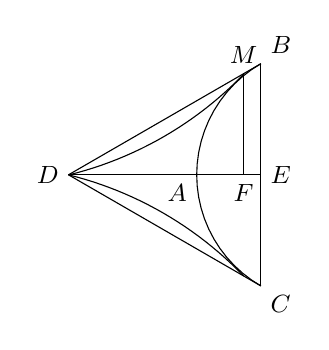
\begin{tikzpicture}[scale=0.9]
				\draw (-1.592,0.)-- (1.123,1.568);
				\draw (1.123,1.568)-- (1.123,-1.568);
				\draw (1.123,-1.568)-- (-1.592,0);
				\draw [shift={(2.028,0)}] plot[domain=2.094:4.1891,variable=\t]({1.*1.8107218179771583*cos(\t r)+0.*1.8107218179771583*sin(\t r)},{0.*1.8107218179771583*cos(\t r)+1.*1.8107218179771583*sin(\t r)});
				\draw [shift={(-2.82,4.994)}]  plot[domain=4.954772812894923:5.517202699071053,variable=\t]({1.*5.145122693791882*cos(\t r)+0.*5.145122693791882*sin(\t r)},{0.*5.145122693791882*cos(\t r)+1.*5.145122693791882*sin(\t r)});
				\draw [shift={(-2.8279022506987714,-4.994723411507955)}]  plot[domain=4.954772812894923:5.517202699071053,variable=\t]({1.*5.145122693791882*cos(\t r)+0.*5.145122693791882*sin(\t r)},{0.*5.145122693791882*cos(\t r)+-1.*5.145122693791882*sin(\t r)});
				\draw (-1.593,0)-- (1.124,0);
				\draw (0.880,1.427) -- (0.880,0);
				\draw (1.123,1.568) node [above right] {\small $B$};
				\draw (1.123,-1.568) node [below right] {\small $C$};
				\draw (-1.592,0) node [left] {\small $D$};
				\draw (1.123,0) node [right] {\small $E$};
				\draw (0.217,0) node [below left] {\small $A$};
				\draw (0.880,1.427) node [above] {\small $M$};
				\draw (0.880,0) node [below] {\small $F$};
				\end{tikzpicture}}
			\fontfamily{cmr}\selectfont
			\caption{Tab. I. Fig. 7.}
		\end{figure}
		\switchcolumn
		\begin{figure}[h]
			\centering
			\par {
				\fontfamily{jkplvos}\selectfont
				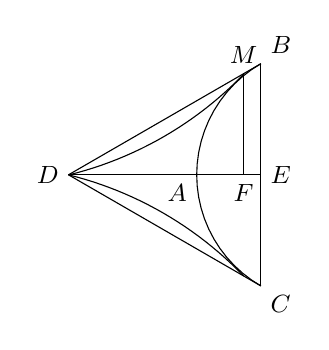
\begin{tikzpicture}[scale=0.9]
				\draw (-1.592,0.)-- (1.123,1.568);
				\draw (1.123,1.568)-- (1.123,-1.568);
				\draw (1.123,-1.568)-- (-1.592,0);
				\draw [shift={(2.028,0)}] plot[domain=2.094:4.1891,variable=\t]({1.*1.8107218179771583*cos(\t r)+0.*1.8107218179771583*sin(\t r)},{0.*1.8107218179771583*cos(\t r)+1.*1.8107218179771583*sin(\t r)});
				\draw [shift={(-2.82,4.994)}]  plot[domain=4.954772812894923:5.517202699071053,variable=\t]({1.*5.145122693791882*cos(\t r)+0.*5.145122693791882*sin(\t r)},{0.*5.145122693791882*cos(\t r)+1.*5.145122693791882*sin(\t r)});
				\draw [shift={(-2.8279022506987714,-4.994723411507955)}]  plot[domain=4.954772812894923:5.517202699071053,variable=\t]({1.*5.145122693791882*cos(\t r)+0.*5.145122693791882*sin(\t r)},{0.*5.145122693791882*cos(\t r)+-1.*5.145122693791882*sin(\t r)});
				\draw (-1.593,0)-- (1.124,0);
				\draw (0.880,1.427) -- (0.880,0);
				\draw (1.123,1.568) node [above right] {\small $B$};
				\draw (1.123,-1.568) node [below right] {\small $C$};
				\draw (-1.592,0) node [left] {\small $D$};
				\draw (1.123,0) node [right] {\small $E$};
				\draw (0.217,0) node [below left] {\small $A$};
				\draw (0.880,1.427) node [above] {\small $M$};
				\draw (0.880,0) node [below] {\small $F$};
				\end{tikzpicture}}
			\fontfamily{cmr}\selectfont
			\caption{Tab. I. Fig. 7.}
		\end{figure}

		\switchcolumn*
		\newpage
		
		\item Accuratius autem in symptomata nostrae curvae triangularis inquiramus, et quoniam pro coordinatis $FT=t$ et $TU=u$ has invenimus formulas:
		\begin{align*}
			t & = \frac{\D S}{\D p}-\frac{p\,\D \D S}{\D p^2}(1+pp)\quad\text{et}\\
			u & = S-\frac{p\,\D S}{\D p}-\frac{\D\D S}{\D p^2}(1+pp)
		\end{align*}
		\par primum observo, rectum $NU$ esse tangentem curvae in punctu $U$, quae cum ad axem sit inclinata angulo $TNU=\phi$, cuius cotangens est $p$, necesse est ut sit $\frac{\D u}{\D t} = \tang \phi = \frac{1}{p}$, unde sit $\D t = p\, \D u$. Est vero per formulas
		\begin{align*}
			\D t &= -\frac{3pp\, \D\D S}{\D p}-\frac{p(1+pp)\, \D^3S}{\D p^2} \quad \text{et}\\
			p\, \D u &= - \frac{3pp \, \D \D S}{\D p} - \frac{p(1+pp)\, \D^3S}{\D p^2}.
		\end{align*}
		ideoque reuera $\D t=p\, \D u$.
		
		\switchenum
		\newpage
		
		\item We onderzoeken meer preciezer de eigenschappen van onze driehoekige kromme, en omdat we voor de coördinaten $FT=t$ en $TU=u$ de formules hebben gevonden:
		\begin{align*}
			t & = \frac{\D S}{\D p}-\frac{p\,\D \D S}{\D p^2}(1+pp)\quad\text{en}\\
			u & = S-\frac{p\,\D S}{\D p}-\frac{\D\D S}{\D p^2}(1+pp)
		\end{align*}
		\par Merk nu eerst op dat de rechte $NU$ rakend is aan de kromme in $U$,die aangezien de hellingshoek met de as $TNU=\phi$ is, die cotangens $p$ heeft, dan is het noodzakelijk dat $\frac{\D u}{\D t} = \tang \phi = \frac{1}{p}$, en dus $\D t = p \, \D u$. Dit volgt ook uit de formules 

		\begin{align*}
			\D t &= -\frac{3pp\, \D\D S}{\D p}-\frac{p(1+pp)\, \D^3S}{\D p^2} \quad \text{en}\\
			p\, \D u &= - \frac{3pp \, \D \D S}{\D p} - \frac{p(1+pp)\, \D^3S}{\D p^2}.
		\end{align*}
		\par Zodat in het echt $\D t=p\, \D u$.
		\switchcolumn*
		
		\begin{figure}[h]
			\centering
			\par {
				\fontfamily{jkplvos}\selectfont
				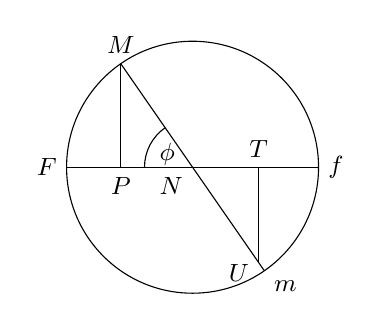
\begin{tikzpicture}[scale=0.8]
				\draw (124.73955121402813:0.7631107015839075) arc (124.73955121402813:180.:0.7631107015839075);
				\draw (0,0) circle (2cm);
				\draw (-1.1396938257701044,1.643501744295242)-- (1.1396938257701044,-1.643501744295242);
				\draw (1.0499141426476895,-1.5140344588914103)-- (1.0499141426476895,0.);
				\draw (-1.1396938257701044,0.)-- (-1.1396938257701044,1.643501744295242);
				\draw (-2,0)-- (2,0);
				
				\draw (0,0) node [below left] {\small $N$};
				\draw (-2,0) node [left] {\small $F$};
				\draw (2,0) node [right] {\small $f$};
				\draw (-1.1396938257701044,1.643501744295242) node [above] {\small $M$};
				\draw (1.1396938257701044,-1.643501744295242) node [below right] {\small $m$};
				\draw (-1.1396938257701044,0.) node [below] {\small $P$};
				\draw (1.0499141426476895,-1.5140344588914103) node [below left,yshift=3pt] {\small $U$};
				\draw (1.0499141426476895,0.) node [above] {\small $T$};
				\draw (-0.4,0.2) node {\small $\phi$};
				\end{tikzpicture}}
			\fontfamily{cmr}\selectfont
			\caption{Tab. I. Fig. 6.}
		\end{figure}
		\switchcolumn
		\begin{figure}[h]
			\centering
			\par {
				\fontfamily{jkplvos}\selectfont
				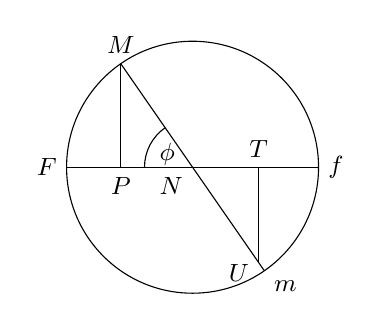
\begin{tikzpicture}[scale=0.8]
				\draw (124.73955121402813:0.7631107015839075) arc (124.73955121402813:180.:0.7631107015839075);
				\draw (0,0) circle (2cm);
				\draw (-1.1396938257701044,1.643501744295242)-- (1.1396938257701044,-1.643501744295242);
				\draw (1.0499141426476895,-1.5140344588914103)-- (1.0499141426476895,0.);
				\draw (-1.1396938257701044,0.)-- (-1.1396938257701044,1.643501744295242);
				\draw (-2,0)-- (2,0);
				
				\draw (0,0) node [below left] {\small $N$};
				\draw (-2,0) node [left] {\small $F$};
				\draw (2,0) node [right] {\small $f$};
				\draw (-1.1396938257701044,1.643501744295242) node [above] {\small $M$};
				\draw (1.1396938257701044,-1.643501744295242) node [below right] {\small $m$};
				\draw (-1.1396938257701044,0.) node [below] {\small $P$};
				\draw (1.0499141426476895,-1.5140344588914103) node [below left,yshift=3pt] {\small $U$};
				\draw (1.0499141426476895,0.) node [above] {\small $T$};
				\draw (-0.4,0.2) node {\small $\phi$};
				\end{tikzpicture}}
			\fontfamily{cmr}\selectfont
			\caption{Tab. I. Fig. 6.}
		\end{figure}


		\switchcolumn*
		
		\item Quia igitur est $\D t=p \,\D u$, iisdem casibus, quibus sit $\frac{\D t}{\D p}=0$, etiam fiet $\frac{\D u}{\D p}= 0$; unde patet, ubicunque abscissa $t$ fuerit vel maxima vel minima, ibidem quoque fore applicatam maximam vel minimam, quae propietas utique in cuspides convenit. Ex quo colligimus, ubicunque ambae coordinatae $p$ et $q$ simul fiunt vel maximae vel minimae, ibi quoque existere cuspides nostrae curvae; quare cum curva habeat tres cuspides, in tribus quoque locis tam $t$ quam $u$ maximum fieri necesse est.
		
		\switchenum
		\item Omdat het zo is dat $\D t=p\, \D u$, de gevallen waarbij het zo is dat $\frac{\D t}{\D p}=0$, en is het ook zo dat $\frac{\D u}{\D p}= 0$; het is dus duidelijk dat, wanneer de abscis $t$ ofwel maximaal ofwel minimaal is, op dezelfde plaats maximaal ofwel minimaal zal zijn, wat de eigenschappen in de spitsen doet samenvallen. Van wat we verzamelen, zijn beide coördinaten $p$ en $q$ dus gelijktijdig ofwel maximaal ofwel minimaal, daar bestaan dan ook de spitsen van onze krommen; en gezien de kromme 3 spitsen hebben, moeten zowel $t$ als $u$ in 3 plaatsen maximaal zijn.



		\switchcolumn*
		
		\item Imprimis autem hic notatu dignum occurrit, nostram curva triangularem esse rectificabilem, quippe cuius arcu aequalis est radio osculi $MU$ curvae orbiformis, unde est nata. Videmus autem esse
		\begin{align*}
			NU &= r = -\frac{\D \D S}{\D p^2}(1+pp)^\frac{3}{2}-\frac{p\,\D S}{\D p}\sqrt{1+pp}\\
			& +S\sqrt{1+pp}; \quad \text{at} \quad MN = y\sqrt{1+pp}\\
			&= \frac{p\, \D S\sqrt{1+pp}}{\D p}-S\sqrt{1+pp},
		\end{align*}
		
		unde sit radius osculi
		
		\[
			MU = -\frac{\D \D S}{\D p^2}(1+pp)^\frac{3}{2},
		\]
		\par qui ergo longitudinem nostrae curvae triangularis exprimit; id quod etiam patet ex proprietate supra observata, quod sit $\D t = p\, \D u$, unde fit elementum curvae
		
		\[
			\sqrt{\D t^2+\D u^2} = \D u\sqrt{1+pp} = -\frac{3p\, \D S}{\D p}\sqrt{1+pp}-\frac{\D^3S}{\D p^2}(1+pp)^\frac{3}{2}
		\]
		cuius integrale manifesto est
		\[
			-\frac{\D \D S}{\D p^2}(1+pp)^\frac{3}{2}.
		\]
		
		\switchenum
		\item In het bijzonder wees erop gewezen dat het voldoende is, onze driehoekige kromme te herleiden, aangezien ze gelijk is aan de kromtestraal $MU$ van onze orbiforme kromme, en eruit geboren wordt. We zien dat
		\begin{align*}
			NU &= r = -\frac{\D \D S}{\D p^2}(1+pp)^\frac{3}{2}-\frac{p\,\D S}{\D p}\sqrt{1+pp}\\
			& +S\sqrt{1+pp}; \quad \text{bij}\\
			MN & = y\sqrt{1+pp} = \frac{p\, \D S\sqrt{1+pp}}{\D p}-S\sqrt{1+pp},
		\end{align*}
		en de kromtestraal
		\[
			MU = -\frac{\D \D S}{\D p^2}(1+pp)^\frac{3}{2},
		\]
		die de lengte van onze driehoekige kromme uitdrukt; het is ook duidelijk van de observaties uit de bovenstaande eigenschap dat $\D t = p\, \D u$, en dus begint de kromme 
		\[
			\sqrt{\D t^2+\D u^2} = \D u\sqrt{1+pp} = -\frac{3p\, \D S}{\D p}\sqrt{1+pp}-\frac{\D^3S}{\D p^2}(1+pp)^\frac{3}{2}
		\]
		waarbij de integraal duidelijk gegeven is door
		\[
			-\frac{\D \D S}{\D p^2}(1+pp)^\frac{3}{2}.
		\]

		\switchcolumn*
		
		\item Quoniam hic tantum curvas triangulares investigare instituimus, parum solliciti, utrum sint rectificabiles nec ne, dummodo fuerint algebraicae: hac conditione omissa simpliciores formulas pro coordinatis $t$ et $u$ exhibere, atque adeo, sine ullo respectu ad curvas orbiformes habito, directe ex ipsa indole harum curvarum elicere poterimus. Cum enim esse debeat $\D t=p \D u$, erit $t=\int p\,\D u = pu-\int u \,\D p$. Iam statuamus $\int u \,\D p = \Pi$, ita ut fit $u=\frac{\D \Pi}{\D p}$, unde sit $t=\frac{p\,\D \Pi}{\D p}-\Pi$; ubi pro $\Pi$ eiusmodi functiones ipsius $p$ accipi debent, quae nullo casu fiant infinitae, quicunque valores literae $t$ tribuantur, cuiusmodi functiones iam supra descripsimus; tum vero etiam hae functiones $\Pi$ nulla signa radicalia, quae ambiguitatem involuant, involvere debent. Imprimis autem necesse est, ut ambae coordinatae $t$ et $u$ tribus casibus fiant maximae vel minimae, id quod eueniet, si, ob $u=\frac{\D \Pi}{\D p}$, haec aequatio: $\frac{\D\D \Pi}{\D p^2} = 0$, tres habeat radices reales, neque vero plures.

		\switchenum
		\item Omdat we hier enkel driehoekige krommen onderzoeken, maken we ons weinig zorgen, of ze al dan niet herleidbaar zijn, op voorwaarde dat ze algebraïsch zijn: deze voorwaarde laten vallen laat toe meer eenvoudige coördinaten $t$ en $u$ te vinden, en daarvoor, zonder rekening te houden met het liggen in de orbiforme krommen, als direct gevolg van de aard van deze krommen stellen we vast. Aangezien moet gelden dat $\D t = p\, \D u$, zal het zijn dat $t=\int p \, \D u= pu-\int u \, \D p$. Laten we nu $\int u \D p = \Pi$, zodat het is $u = \frac{\D \Pi}{\D p}$, waardoor $t=\frac{p\,\D \Pi}{\D p}-\Pi$; als voor $\Pi$ op deze manier een een functie van $p$ moet worden genomen, dat in geen geval oneindig is \ldots van welke aard functies hierboven reeds werden beschreven; maar zelfs dan heeft de functie $\Pi$ geen worteltekens moeten betrekken, wat gewikkeld is in onzekerheid. Maar bovenal is het noodzakelijk dat, beide coördinaten $t$ en $u$ in drie gevallen maximaal ofwel minimaal zijn, hetgeen tot gevolg heeft dat voor $u=\frac{\D \Pi }{\D p}$, als $\frac{\D \D \Pi}{\D p^2}=0$, drie reële wortels heeft, of echt meer.
		\switchcolumn*
		
		\item Sumamus exempli gratia $\Pi = \frac{a+bp}{1+fp+gpp}$, quae nullo casu fit infinita, si modo fuerit $ff< 4g$, tum autem erit
		\[
			\frac{\D \Pi}{\D p} = \frac{b-af-2agp-bgpp}{(1+fp+gpp)^2} = u
		\]
		hincque
		\[
			t = \frac{-a-2afp-3agp^2-2bgp^3}{(1+fp+gpp)^2}.
		\]
		\par Ut iam ternas cuspides definiamus, consideremus aequationem $\frac{\D u}{\D p} = 0$, quod quo facilius fieri possit ponamus
		\[
			u  =  \frac{A+Bp+Cpp}{(1+fp+gpp)^2},
		\]
		ita ut sit $A=b-af, B=-2ag; C=-bg$; tunc vero hinc reperitur sequens aequatio:
		\[
			B-2Af+(2C-Bf-4Ag)p-3Bgpp-2Cgp^3 = 0
		\]
		cuius tres radices nobis ternas cuspides monstrabunt.
		
		\switchenum
		\item Laten we bijvoorbeeld $\Pi = \frac{a+bp}{1+fp+gpp}$, dat in geen geval oneindig is, als het maar $ff< 4g$, dan zal
		\[
			\frac{\D \Pi}{\D p} = \frac{b-af-2agp-bgpp}{(1+fp+gpp)^2} = u
		\]
		wat leidt tot
		\[
			t = \frac{-a-2afp-3agp^2-2bgp^3}{(1+fp+gpp)^2}.
		\]
		\par Om de drie spitsen te definiëren, 	overwegen we de vergelijking $\frac{\D u}{\D p}=0$, wat we eenvoudiger kunnen maken door 
		\[
			u  =  \frac{A+Bp+Cpp}{(1+fp+gpp)^2},
		\]
		\par waarbij $A=b-af; B= -2ag; C=-bg$; dan vindt men hier de volgende vergelijking:
		\[
			B-2Af+(2C-Bf-4Ag)p-3Bgpp-2Cgp^3 = 0
		\]
		\par waarvan de drie wortels onze drie spitsen onthullen.
		
		\switchcolumn*
		
		\item Ponamus iam huius aequationis radices esse: I\degree. $p=\alpha$, II\degree. $p=\beta$ ac III\degree. $p=\gamma$, sive aequemus formulam inventum huic producto:
		\[
			2Cg(a-p)(\beta-p)(\gamma-p)
		\]
		\par quod evolutum praebet
		\[
			2Cg\alpha \beta \gamma - 2Cg(\alpha \gamma+\alpha \gamma+\beta \gamma)p+2Cg(\alpha+\beta+\gamma)pp - 2Cgp^3
		\]
		\par quae forma, inventae aequata, sequentes tres producit determinationes:
		\begin{align*}
			\text{I}\degree. \;& B-2Af = 2Cg\alpha\beta\gamma;\\
			\text{II}\degree. \; & 2C-Bf-4Ag = -2Cg(\alpha \beta +\alpha \gamma+\beta \gamma);\\
			\text{III}\degree. \; & -3Bg; = 2Cg(\alpha+\beta+\gamma);
		\end{align*}
		
		\par ex quarum tertia fit $B=-\frac{2}{3}C(\alpha+\beta+\gamma)$; ex prima vero
		\[
			A = -\frac{1}{3f}C(\alpha+\beta+\gamma)-\frac{1}{f}Cg\alpha \beta \gamma,
		\]
		qui valores in secunda substituti praebent
		\[
			2C+\frac{(2ff+4g)}{3f}C(\alpha+ \beta + \gamma)+\frac{4g}{f}Cg\alpha \beta \gamma  = -2Cg(\alpha \beta + \alpha \gamma+\beta \gamma)
		\]
		quae aequatio, per $\frac{3f}{2C}$ multiplicata, abit in hanc:
		\[
			3f+(ff+2g)(\alpha+\beta+\gamma)+6gg\alpha  \beta \gamma = -3fg(\alpha \beta + \alpha \gamma + \beta \gamma)
		\]
		haecque aequationes omnes continent determinationes, quibus nostro proposito satisfit.
		
		\switchenum
		\item Laten we veronderstellen dat de wortels van deze vergelijking al gegeven zijn: $p=\alpha$, II\degree. $p=\beta$ ac III\degree. $p=\gamma$, of gelijk aan de formule gevonden door het product
		\[
			2Cg(a-p)(\beta-p)(\gamma-p)
		\]
		
		\newpage
		
		\par die als ontwikkeling biedt
		
		\[
			2Cg\alpha \beta \gamma - 2Cg(\alpha {\color{red}\beta\;}+\alpha \gamma+\beta \gamma)p+2Cg(\alpha+\beta+\gamma)pp - 2Cgp^3
		\]
		\par welke de vorm, gevonden uit de vergelijking, de volgende drie bepalingen produceert:
		\begin{align*}
			\text{I}\degree. \;& B-2Af = 2Cg\alpha\beta\gamma;\\
			\text{II}\degree. \; & 2C-Bf-4Ag = -2Cg(\alpha \beta +\alpha \gamma+\beta \gamma);\\
			\text{III}\degree. \; & -3Bg; = 2Cg(\alpha+\beta+\gamma);
		\end{align*}
		\par uit de derde volgt $B=-\frac{2}{3}C(\alpha+\beta+\gamma)$; van de eerste echter
		\[
			A = -\frac{1}{3f}C(\alpha+\beta+\gamma)-\frac{1}{f}Cg\alpha \beta \gamma,
		\]
		\par welke waarden in de tweede vervangen worden geeft:
		\[
			2C+\frac{(2ff+4g)}{3f}C(\alpha+ \beta + \gamma)+\frac{4g}{f}Cg\alpha \beta \gamma  = -2Cg(\alpha \beta + \alpha \gamma+\beta \gamma)
		\]
		\par Deze vergelijking met $\frac{3f}{2C}$ vermenigvuldigen, wijzigt naar:
		\[
			3f+(ff+2g)(\alpha+\beta+\gamma)+6gg\alpha  \beta \gamma = -3fg(\alpha \beta + \alpha \gamma + \beta \gamma)
		\]
		\par de vergelijkingen hier bevatten alle bepalingen, om aan ons doel te voldoen.		
		
		\switchcolumn*
		
		\item Antequam hanc determinationem iu genere ulterius prosequamur, evoluamus casum specialem, quo 
		\begin{align*}
			&\gamma = 0 \text{ et } \beta = -\alpha, \quad \text{unde sit} \quad \alpha\beta\gamma = 0;\\
			&\quad \alpha\beta+\alpha \gamma+\beta \gamma = -\alpha^2 \quad \text{et} \quad \alpha+\beta+ \gamma = 0,
		\end{align*}
		\par eritque postrema aequatio $3f = 3\alpha \alpha f g$, sive $f=\alpha \alpha fg$; unde sequitur vel $f= 0$, vel $g= \frac{1}{\alpha \alpha}$. Consideremus primo casum $f=0$, fietque $A = -\frac{0}{0}$, unde littera $A$ non determinatur, vel potius fit $A = 0$, porroque $B=0$, unde colligitur $b=0$, sive etiam $b$ non determinatur; tum vero erit $a=0$. Quia autem aequationem postremam per $f$ multiplicauimus, hic valor $f=0$ lubricus est habendus. Sumamus igitur alterum valorem $g= \frac{1}{\alpha \alpha}$, et quia debet esse $ff<4g$, sequitur esse debere $f< \frac{2}{\alpha}$; hinc vero fiet $A=0$ et $B=0$, ideoque $b-af = 0$, et $-2ag = 0$, unde sit $a = 0$.
		
		\switchenum
			\item Alvorens we de algemene bespreking van de bepalingen voortzetten, evalueren we het speciale geval, waarbij
		\begin{align*}
			&\gamma = 0 \text{ et } \beta = -\alpha, \quad \text{waardoor} \quad \alpha\beta\gamma = 0;\\
			&\quad \alpha\beta+\alpha \gamma+\beta \gamma = -\alpha^2 \quad \text{en} \quad \alpha+\beta+ \gamma = 0,
		\end{align*}
		zo wordt de laatste vergelijking  $3f = 3\alpha \alpha f g$,  of $f=\alpha \alpha fg$; hieruit volgt ofwel $f=0$, ofwel $g=\frac{1}{\alpha \alpha}$. Beschouw het eerste geval, $f=0$, en dus $A = -\frac{0}{0}$, waarbij de letter $A$ niet kan worden bepaald, ofwel wordt eerder $A=0$, gezien ook $B=0$, vandaar ook $b=0$, of zelfs $b$ niet bepaald;  maar dan zal $a=0$. Aangezien we de finale vergelijking met $f$ vermenigvuldigd hebben, wordt de waarde $f=0$ als \textbf{glad} beschouwd. Laten we de tweede waarde bekijken $g=\frac{1}{\alpha \alpha}$, en gezien het moet zijn dat $ff<4g$, moet worden gevolgd $f< \frac{2}{\alpha}$; maar hieruit zal $A=0$ en $B=0$, daardoor is $b-af=0$, en $-2a g = 0$, en is $a=0$.

		\switchcolumn*
		
		\item Sufficiat autem haec in genere indicasse, et considermus potius casum magis determinatum, sumendo 
		\begin{align*}
			\Pi &= \frac{bp}{\alpha \alpha + pp},\quad \text{unde fit} \quad \frac{\D \Pi}{\D p} =u = \frac{b(\alpha\alpha- pp)}{(\alpha\alpha+pp)^2}\quad \text{et}\\
			&t = \frac{2bp^3}{(\alpha \alpha+pp)^2}.
		\end{align*}

		\par Quod si iam pro cuspidibus faciamus $\frac{\D u}{\D p}=0$, nascitur haec aequatio: $p^3-3\alpha \alpha p = 0$, cuius ternae radices sunt
		\[
			\text{I}\degree.\; p=0;\quad \text{II}\degree.\; p=+\alpha\sqrt{3};\quad  \text{III}\degree.\; p=-\alpha \sqrt{3}
		\]
		\par pro quarum prima habebimus $t=0$ et $u=\frac{b}{\alpha \alpha}$;
		\par pro secunda:
		\[
			t = \frac{2b\sqrt{3}}{8\alpha} \quad \text{et} \quad u = -\frac{b}{8\alpha \alpha};
		\]
		pro tertia vero:
		\[
			t = \frac{-3b\sqrt{3}}{8\alpha} \quad \text{et} \quad u = -\frac{b}{8\alpha \alpha},
		\]
		unde curva habebit formam in figura 8 delineatam, ubi est
		\begin{align*}
			FB &= \frac{b}{\alpha\alpha}, FG = FH = \frac{3b\sqrt{3}}{8\alpha} \qquad\text{ac}\\
			&GC=HD=\frac{-b}{8\alpha \alpha}
		\end{align*}
		sicque ternae cuspides erunt in punctis $B, C, D$, ac ductis chordis erit
		\[
			BC = BD = \frac{3b\sqrt{3}(1+ \alpha \alpha)}{8\alpha \alpha} \quad \text{et} \quad CD = \frac{3b\sqrt{3}}{4\alpha},
		\]
		\par ita ut haec figura triangularis triangulum isosceles exhibeat.
		
		\switchenum
		\item Laat het genoeg zijn deze in het algemene geval bekend te maken, en laten we eerder een meer bepaalde vorm beschouwen, neem
		\begin{align*}
			\Pi &= \frac{bp}{\alpha \alpha + pp},\quad \text{waardoor} \quad \frac{\D \Pi}{\D p} =u = \frac{b(\alpha\alpha- pp)}{(\alpha\alpha+pp)^2}\quad \text{en}\\
			&t = \frac{2bp^3}{(\alpha \alpha+pp)^2}.
		\end{align*}
		\par Maar als je voor de spits maakt $\frac{\D u}{\D p}=0$ hieruit wordt de vergelijking geboren: $p^3-3\alpha \alpha p = 0$, waarvan de wortels zijn
		\[
			\text{I}\degree.\; p=0;\quad \text{II}\degree.\; p=+\alpha\sqrt{3};\quad  \text{III}\degree.\; p=-\alpha \sqrt{3}
		\]
		\par voor de eerste hebben we $t=0$ en $u=\frac{b}{\alpha \alpha}$;
		\par voor de tweede:
		\[
			t = \frac{2b\sqrt{3}}{8\alpha} \quad \text{en} \quad u = -\frac{b}{8\alpha \alpha};
		\]
		\par voor de derde waarde:
		\[
			t = \frac{-3b\sqrt{3}}{8\alpha} \quad \text{en} \quad u = -\frac{b}{8\alpha \alpha},
		\]
		\par waarbij de kromme de vorm geschetst in figuur 8 aanneemt, waar
		\begin{align*}
			FB &= \frac{b}{\alpha\alpha}, FG = FH = \frac{3b\sqrt{3}}{8\alpha} \qquad\text{en}\\
			&GC=HD=\frac{-b}{8\alpha \alpha}
		\end{align*}
		\par zodat de drie spitsen ontstaan in $B, C, D$, en de verbonden koorden zijn
		\[
			BC = BD = \frac{3b\sqrt{3}(1+ \alpha \alpha)}{8\alpha \alpha} \quad \text{en} \quad CD = \frac{3b\sqrt{3}}{4\alpha},
		\]
		\par en uit deze driehoekige figuur ontstaat een gelijkbenige driehoek.
	
		\switchcolumn*
		
		\begin{figure}[h]
			\centering
			\par {
				\fontfamily{jkplvos}\selectfont
				\begin{tikzpicture}[rotate=180, scale=1]
				
				\end{tikzpicture}}
			\fontfamily{cmr}\selectfont
			\caption{Tab. I. Fig. 8.}
		\end{figure}
		\switchcolumn
		\begin{figure}[h]
			\centering
			\par {
				\fontfamily{jkplvos}\selectfont
				\begin{tikzpicture}[rotate=180, scale=1]
				
				\end{tikzpicture}}
			\fontfamily{cmr}\selectfont
			\caption{Tab. I. Fig. 8.}
		\end{figure}
	
		\switchcolumn*
		
		\item Evoluamus simili modo casum $\Pi = \frac{a}{\alpha\alpha + pp}$, unde sit
		\[
			\frac{\D \Pi}{\D p} = u = -\frac{2a p}{(\alpha \alpha + pp)^2}, \quad \text{hincque}\quad t = -\frac{a(\alpha \alpha+ 3pp)}{(\alpha \alpha +pp)^2}.
		\]
		\par Nunc pro cuspidibus fiat
		\[
			\frac{\D u}{ \D p} = -\frac{2a(\alpha\alpha- 3pp)}{(\alpha\alpha+ pp)^3} = 0,
		\]
		\par quae aequatio tantum duas praebet radices
		\[
			p = +\frac{\alpha}{\sqrt{3}} \quad \text{et} \quad p = -\frac{\alpha}{\sqrt{3}};
		\]
		tertia autem radix est $p=\infty$. Hinc igitur pro prima cuspide, quae sit ubi $p=\infty$, fit $t=0$ et $u=0$, sicque haec cuspis $B$ cadit in ipsum punctum $F$. Pro secunda cuspide sumatur
		\[
			p = \frac{\alpha}{\sqrt{3}}, \quad \text{eritque}\quad t = \frac{-9a}{8\alpha \alpha} \quad \text{et} \quad u=-\frac{3a \sqrt{3}}{8\alpha^3}.
		\]
		\par Pro tertia cuspide sit
		\[
			p = -\frac{\alpha}{\sqrt{3}}, \quad \text{erit} \quad t = -\frac{9a}{8\alpha \alpha} \quad \text{et} \quad u=+\frac{3a \sqrt{3}}{8\alpha^3}.
		\]
		\par Sumto igitur $FG = \frac{9\alpha}{8\alpha \alpha}$ binae reliquae cuspides erunt in $C$ et $D$, ita ut sit $GC = GD = \frac{3a \sqrt{3}}{8\alpha^3}$, ideoque earum distantia
		\begin{align*}
			CD& = \frac{3a \sqrt{3}}{4\alpha^3}, \quad \text{unde colligitur}\\
			BC &= BD = \frac{3a \sqrt{9\alpha \alpha+3}}{8\alpha^3}
		\end{align*}
		\par sicque erit
		\[
			CD : BC = 2:\sqrt{3\alpha\alpha + 1}
		\]
		\par ex quo patet, casu $\alpha = 1$ triangulum fore aequilaterum.
		
		\switchenum
		\item Laten we op een gelijkaardige manier het geval $\Pi = \frac{a}{\alpha\alpha + pp}$ evalueren, waarbij
		\[
			\frac{\D \Pi}{\D p} = u = -\frac{2a p}{(\alpha \alpha + pp)^2}, \quad \text{waardoor}\quad t = -\frac{a(\alpha \alpha+ 3pp)}{(\alpha \alpha +pp)^2}.
		\]
		\par Nu voor de spitsen wordt
		\[
			\frac{\D u}{ \D p} = -\frac{2a(\alpha\alpha- 3pp)}{(\alpha\alpha+ pp)^3} = 0,
		\]
		\par waarbij de vergelijking alleen twee wortels heeft
		\[
			p = +\frac{\alpha}{\sqrt{3}} \quad \text{en} \quad p = -\frac{\alpha}{\sqrt{3}};
		\]
		\par en een andere derde wortel is $p=\infty$. Daarom geeft dit hier een eerste spits, dat is waar $p=\infty$, is $t=0$ en $u=0$, zodat het punt $B$ samenvalt met het punt $F$. De tweede spits wordt bekomen
		\[
			p = -\frac{\alpha}{\sqrt{3}}, \quad \text{en dan} \quad t = -\frac{9a}{8\alpha \alpha} \quad \text{en} \quad u=-\frac{3a \sqrt{3}}{8\alpha^3}.
		\]
		\par Voor de derde spits is
		\[
			p = -\frac{\alpha}{\sqrt{3}}, \quad \text{en dan} \quad t = -\frac{9a}{8\alpha \alpha} \quad \text{en} \quad u=+\frac{3a \sqrt{3}}{8\alpha^3}.
		\]
		\par Met $FG = \frac{9a}{8\alpha \alpha}$ zijn de twee resterende punten $C$ en $D$, zodat het kan dat $GC=GD=\frac{3a\sqrt{3}}{8\alpha^3}$, waardoor de afstand
		\begin{align*}
			CD& = \frac{3a \sqrt{3}}{4\alpha^3}, \quad \text{vandaar dat}\\
			BC &= BD = \frac{3a \sqrt{9\alpha \alpha+3}}{8\alpha^3}
		\end{align*}
		\par hieruit is het duidelijk dat
		\[
			CD : BC = 2:\sqrt{3\alpha\alpha + 1}
		\]
		\par uit het geval, $\alpha =1$ zou het een gelijkzijdige driehoek zijn.

		\switchcolumn*
		
		\begin{figure}[h]
			\centering
			\par {
				\fontfamily{jkplvos}\selectfont
				\begin{tikzpicture}[rotate=180, scale=1]
				
				\end{tikzpicture}}
			\fontfamily{cmr}\selectfont
			\caption{Tab. I. Fig. 9.}
		\end{figure}
		\switchcolumn
		\begin{figure}[h]
			\centering
			\par {
				\fontfamily{jkplvos}\selectfont
				\begin{tikzpicture}[rotate=180, scale=1]
				
				\end{tikzpicture}}
			\fontfamily{cmr}\selectfont
			\caption{Tab. I. Fig. 9.}
		\end{figure}

		\switchcolumn*	
		
		\item Quod si ergo ambo casus praecedentes combinentur, ita ut statuatur $\Pi=\frac{a + bp}{\alpha \alpha + pp}$, tum tam abscissa $t$ quam applicata $u$ aequabitur summae ambarum praecedentium formularum, ita ut sit
		\[
			t = \frac{2bp^3 - a(\alpha \alpha + 3pp)}{(\alpha \alpha + pp)^2} \quad \text{et} \quad u = \frac{b(\alpha \alpha - pp)-2ap}{(\alpha \alpha + pp)^2};
		\]
		\par unde si pro cuspidibus inveniendis ponamus $\frac{\operatorname{d}u}{\operatorname{d}p} = 0$, habebimus hanc aequationem:
		\begin{align*}
			&2bp^3-6b\alpha \alpha p -2a \alpha \alpha +6a pp = 0, \quad \text{sive} \quad bp^3+3app\\
			&\qquad-3b\alpha \alpha p - a\alpha \alpha = 0,
		\end{align*}
		\par cuius ergo ternas radices quaeri oportet, quod cum per regulam \textit{Cardani} difficulter praestetur, trisectione anguli utamur, quem in finem fingamus esse $p=r+s\cosg \phi$ eritque
		\begin{align*}
			pp & = rr + \frac{1}{2}ss +2rs \cosg\phi + \frac{1}{2}ss \cosg 2\phi \quad \text{et}\\
			p^3 & = r^3+\frac{2}{3}rss + (3rrs+\frac{3}{4}s^3)\cosg \phi + \frac{3}{2} rss \cosg 2\phi+\frac{1}{4}s^3\cosg 3\phi
		\end{align*}
		\par quibus valoribus substitutis aequatio nostra transmutabitur in sequentem:
		\begin{align*}
			&+br^3+3brrs \cosg \phi + \frac{3}{2}brss \cosg 2\phi+ \frac{1}{4}bs^3\cosg 3\phi\\
			&+\frac{3}{2}brss + \frac{3}{4}bs^3\cosg \phi + \frac{3}{2}ass \cosg 2\phi\\
			&+3arr + 6ars \cosg \phi\\
			&+\frac{3}{2}ass - 3b\alpha \alpha \cosg \phi\\
			&-3b\alpha \alpha r\\
			&-a \alpha \alpha.
		\end{align*}
		\par Nunc definiantur litterae $r$ et $s$ ita, ut membra intermedia, tam $\cosg \phi$ quam $\cosg 2\phi$ involventia, seorsim evanescant, unde hae duae aequationes oriuntur:
		\begin{align*}
			\text{I}\degree.\; &3brrs + \frac{3}{4}bs^3+6ars-3b\alpha \alpha s = 0;\\
			\text{II}\degree.\;& \frac{3}{2}brss+\frac{3}{2}ass = 0;
		\end{align*}
		\par ex quarum, posteriore fit $r=-\frac{a}{b}$, qui valor in priore substitutus dat
		\begin{align*}
			&\frac{3aas}{b}+\frac{3}{4}bs^3-\frac{6aas}{b}-3b\alpha \alpha s = 0, \quad \text{unde fit}\\
			&ss = \frac{4(bb\alpha \alpha + aa)}{bb}, \quad \text{ideoque} \quad s = \frac{2\sqrt{bb\alpha \alpha + aa}}{b}.
		\end{align*}
		\par Hi iam valores in nostra aequatione substituantur, fietque
		\[
			\frac{2a^3}{bb}+2a\alpha \alpha + \frac{1}{4}bs^3\cosg 3\phi = 0,
		\]
		\par unde fit
		\[
			\cosg 3\phi = - \frac{3a(aa + bb\alpha \alpha)}{b^3s^3} =-\frac{a}{\sqrt{aa+bb\alpha \alpha}}.
		\]
		\par Quaeratur igitur angulus $\omega$, cuius Cosinus sit
		\[
			= -\frac{a}{\sqrt{aa+bb\alpha \alpha}},
		\]
		qui Cosinus cum etiam conveniat angulis $-\omega$; $2\pi - \omega$; item $2\pi + \omega$, habebimus sequentes valores:
		\begin{align*}
			&\text{I}\degree.\;3\phi = \omega, \quad \text{II}\degree.\; 3\phi = -\omega, \quad \text{III}\degree.\; 3\phi = 2\pi - \omega, \\
			&\qquad \text{IV}\degree.\; \quad \text{et} \quad 3\phi = 2\pi+\omega
		\end{align*}
		\par unde omisso secundo valore, quippe qui a primo non discrepat, tres valores pro angulo $\phi$ erunt
		\[
			\text{I}\degree.\; \phi = \frac{1}{3}\omega, \quad \text{II}\degree.\; 120\degree - \frac{1}{3}\omega \quad \text{et}\quad  \phi = 120\degree +\frac{1}{3}\omega,
		\]
		\par quibus inventis terni valores litterae $p$ erunt
		\begin{align*}
			\text{I\textsuperscript{us}.}\;  p &= -\frac{a}{b}+\frac{2\sqrt{bb\alpha \alpha + aa}}{b} \cosg \frac{1}{3} \omega,\\
			\text{II\textsuperscript{us}.}\; p &= -\frac{a}{b}+\frac{2\sqrt{bb\alpha \alpha + aa}}{b} \cosg (120\degree - \frac{1}{3}\omega),\\
			\text{III\textsuperscript{us}.}\; p & = -\frac{a}{b}+\frac{2\sqrt{bb\alpha \alpha+aa}}{b} \cosg (120\degree + \frac{1}{3}\omega).
		\end{align*}
		
		\switchenum
		\item Daarom kunnen we de voorgaande zaken combineren, en dus geldt $\Pi = \frac{a+bp}{\alpha\alpha+pp}$, evenals kunnen we dit toepassen op de abscissen $t$ en $u$ gelijk aan de de som van de voorgaande formules, zodat het is
		\[
			t = \frac{2bp^3 - a(\alpha \alpha + 3pp)}{(\alpha \alpha + pp)^2} \quad \text{en} \quad u = \frac{b(\alpha \alpha - pp)-2ap}{(\alpha \alpha + pp)^2};
		\]
		\par en als voor de spitsen wordt gezet $\frac{\D u}{\D p}=0$, hebben we deze vergelijking
		\begin{align*}
			&2bp^3-6b\alpha \alpha p -2a \alpha \alpha +6a pp = 0, \quad \text{of} \quad bp^3+3app\\
			&\qquad-3b\alpha \alpha p - a\alpha \alpha = 0,
		\end{align*}
		\par het is dus nodig te zoeken naar de drie wortels, maar met de regel van \textit{Cardano} is dit eenvoudig volbracht, om gebruik te maken van een driedelige hoek, die we eindig veronderstellen is $p=r+s+\cosg \phi$, en dan
		\begin{align*}
			pp & = rr + \frac{1}{2}ss +2rs \cosg\phi + \frac{1}{2}ss \cosg 2\phi \quad \text{en}\\
			p^3 & = r^3+\frac{2}{3}rss + (3rrs+\frac{3}{4}s^3)\cosg \phi + \frac{3}{2} rss \cosg 2\phi+\frac{1}{4}s^3\cosg 3\phi
		\end{align*}
		\par waarbij deze waarden substitueren onze vergelijking in de volgende uitdrukking omzet:
		\begin{align*}
			&+br^3+3brrs \cosg \phi + \frac{3}{2}brss \cosg 2\phi+ \frac{1}{4}bs^3\cosg 3\phi\\
			&+\frac{3}{2}brss + \frac{3}{4}bs^3\cosg \phi + \frac{3}{2}ass \cosg 2\phi\\
			&+3arr + 6ars \cosg \phi\\
			&+\frac{3}{2}ass - 3b\alpha \alpha \cosg \phi\\
			&-3b\alpha \alpha r\\
			&-a \alpha \alpha.
		\end{align*}
		\par Definieer nu de letters $r$ en $s$ op een zodanige manier, dat de leden van de tussenproducten, betrokken aan $\cosg \phi$ en $\cosg 2\phi$, afzonderlijk verdwijnen, hetgeen tot deze twee vergelijkingen leidt:
		\begin{align*}
			\text{I}\degree.\; &3brrs + \frac{3}{4}bs^3+6ars-3b\alpha \alpha s = 0;\\
			\text{II}\degree.\;& \frac{3}{2}brss+\frac{3}{2}ass = 0;
		\end{align*}
		\par uit de laatste wordt $r=-\frac{a}{b}$, waarvan de waarde in de voormalige vervangen geeft:
		\begin{align*}
			&\frac{3aas}{b}+\frac{3}{4}bs^3-\frac{6aas}{b}-3b\alpha \alpha s = 0, \quad \text{waardoor}\\
			&ss = \frac{4(bb\alpha \alpha + aa)}{bb}, \quad \text{daarom} \quad s = \frac{2\sqrt{bb\alpha \alpha + aa}}{b}.
		\end{align*}
		\par Deze waarden in onze vergelijking vervangen, leidt tot
		\[
			\frac{2a^3}{bb}+2a\alpha \alpha + \frac{1}{4}bs^3\cosg 3\phi = 0,
		\]
		waardoor
		\[
			\cosg 3\phi = - \frac{3a(aa + bb\alpha \alpha)}{b^3s^3} =-\frac{a}{\sqrt{aa+bb\alpha \alpha}}.
		\]
		\par Er wordt dus gevraagd een hoek $\omega$, zodat de Cosinus gegeven is door: 
		\[
			= -\frac{a}{\sqrt{aa+bb\alpha \alpha}},
		\]
		hij is het ook eens met de Cosinus van een hoek $-\omega$; $2\pi - \omega$; en ook $2\pi+\omega$, we hebben de volgende waarden:
		\begin{align*}
			&\text{I}\degree.\;3\phi = \omega, \quad \text{II}\degree.\; 3\phi = -\omega, \quad \text{III}\degree.\; 3\phi = 2\pi - \omega, \\
			&\qquad \text{IV}\degree.\; \quad \text{et} \quad 3\phi = 2\pi+\omega
		\end{align*}
		
		\par waarvan we de waarde van de tweede hebben weggelaten, aangezien hij niet sterk verschilt met de eerste, de drie waarden voor de hoek $\phi$ zijn dus
		\[
			\text{I}\degree.\; \phi = \frac{1}{3}\omega, \quad \text{II}\degree.\; 120\degree - \frac{1}{3}\omega \quad \text{en}\quad  \phi = 120\degree +\frac{1}{3}\omega,
		\]
		\par de drie gevonden waarden voor de letter $p$ zijn
		\begin{align*}
			\text{I\textsuperscript{us}.}\;  p &= -\frac{a}{b}+\frac{2\sqrt{bb\alpha \alpha + aa}}{b} \cosg \frac{1}{3} \omega,\\
			\text{II\textsuperscript{us}.}\; p &= -\frac{a}{b}+\frac{2\sqrt{bb\alpha \alpha + aa}}{b} \cosg (120\degree - \frac{1}{3}\omega),\\
			\text{III\textsuperscript{us}.}\; p & = -\frac{a}{b}+\frac{2\sqrt{bb\alpha \alpha+aa}}{b} \cosg (120\degree + \frac{1}{3}\omega).
		\end{align*}
		
		\switchcolumn*
		
		\item His casibus evolutis revertamur ad quaestionem nostram generalem, qua eiusmodi curvae triangulares quaeruntur, in quibus pro cuspidibus littera $p$ ternos datos obtineat valores, scilicet: $p=\alpha, p=\beta$ et $p=\gamma$. Nunc autem primo ponamus brevitatis gratia $\alpha+\beta+\gamma = \zeta$; $\alpha\beta + \alpha \gamma + \beta \gamma = \eta$ et $\alpha \beta \gamma = \theta$, et tres aequationes adimplendae erunt
		\begin{align*}
			\text{I}\degree. \;&B -2Af = 2Cg\theta\\
			\text{II}\degree. \;& 2C-Bf-4Ag = -2Cg\eta\\
			\text{III}\degree. \;& -3Bg = 2Cg\zeta.
		\end{align*}
		\par Cum igitur esset
		\[
			A=b=af, B=-2ag \quad \text{et}\quad C= -bg,
		\]
		\par hinc ternae nostrae aequationes erunt
		\begin{align*}
			\text{I}\degree. \;& -ag -bg+aff = -bgg\theta\\
			\text{II}\degree. \;& 3b +3af = bg\eta\\
			\text{III}\degree. \;& 3a=-b\zeta;		
		\end{align*}
		\par ex quibus statim ternos valores pro fractione $\frac{a}{b}$ nanciscimur, qui sunt:
		\[
			\text{I}\degree. \frac{a}{b} = \frac{f-gg\theta}{ff-g},\quad  \text{II}\degree. \frac{a}{b} = \frac{g\eta + 3}{3f} \quad \text{et}\quad \text{III}\degree. \frac{a}{b} = -\frac{\zeta}{3}.
		\]
		
		\switchenum
		\item Na het ontwikkelen van deze gevallen keren we terug naar onze algemene vraag, zodat ik zoek naar driehoekige krommen, waarbij voor de spitsen de letter $p$ drie waarden verkrijgt, namelijk $p=\alpha, p=\beta$ en $p=\gamma$. $\alpha\beta + \alpha \gamma + \beta \gamma = \eta$ et $\alpha \beta \gamma = \theta$. Laat ons nu eerst kortheidshalve verwelkomen  $\alpha+\beta+\gamma = \zeta$; $\alpha\beta + \alpha \gamma + \beta \gamma = \eta$ en $\alpha \beta \gamma = \theta$, en de drie vergelijkingen voldoen aan:
		\begin{align*}
			\text{I}\degree. \;&B -2Af = 2Cg\theta\\
			\text{II}\degree. \;& 2C-Bf-4Ag = -2Cg\eta\\
			\text{III}\degree. \;& -3Bg = 2Cg\zeta.
		\end{align*}
		\par Aangezien derhalve het is
		\[
			A=b\;{\color{red}-}\;af, B=-2ag \quad\text{en}\quad C= -bg,
		\]
		\par hierdoor zijn onze drie vergelijkingen
		\begin{align*}
			\text{I}\degree. \;& -ag -bg+aff = -bgg\theta\\
			\text{II}\degree. \;& -3b +3af = bg\eta\\
			\text{III}\degree. \;& 3a=-b\zeta;		
		\end{align*}
		\par hieruit ontmoeten we onmiddellijk drie waarden voor de breuk $\frac{a}{b}$, die zijn:
		\[
			\text{I}\degree. \frac{a}{b} = \frac{f-gg\theta}{ff-g},\quad  \text{II}\degree. \frac{a}{b} = \frac{g\eta + 3}{3f} \quad \text{en}\quad \text{III}\degree. \frac{a}{b} = -\frac{\zeta}{3}.
		\]
		
		\switchcolumn*
		
		\item Quod si iam horum valorum secundus et tertius inter se aequentur, prodibit $f=-\frac{g\eta -3 }{\zeta}$. Aequetur nunc primus valor etiam tertio, et erit
		\[
			3f-3gg\theta = -ff \zeta + g \zeta,
		\]
		ubi, si loco $f$ valor modo inuentus substituatur, prodibit
		\[
			3g\eta -3gg\zeta \theta = g\zeta \zeta - gg\eta \eta
		\]
		\par quae aequatio per $g$ divisa dat
		\begin{align*}
			&3\eta - 3g\zeta \theta = \zeta \zeta - g\eta \eta, \quad \text{unde concluditur}\\
			&g= \frac{3\eta - \zeta \zeta}{3\zeta \theta - \eta \eta}, \quad \text{hincque porro} \quad f = \frac{\zeta \eta - 9\theta}{3\zeta \theta - \eta \eta}.
		\end{align*}
		
		\switchenum
		\item Als deze tweede en derde waarden aan elkaar gelijk zijn, produceert dit $f=-\frac{g\eta -3}{\zeta}$. Is nu ook de eerste waarde gelijk aan de derde, er geldt
		\[
			3f-3gg\theta = -ff \zeta + g \zeta,
		\]
		en, als hier de ontdekte waarde $f$ wordt gesubstitueerd, produceert dit
		\[
			3g\eta -3gg\zeta \theta = g\zeta \zeta - gg\eta \eta
		\]
		\par deze vergelijking delen door $g$ 
		\begin{align*}
			&3\eta - 3g\zeta \theta = \zeta \zeta - g\eta \eta, \quad \text{en we besluiten}\\
			&g= \frac{3\eta - \zeta \zeta}{3\zeta \theta - \eta \eta}, \quad \text{hetgeen leidt tot} \quad f = \frac{\zeta \eta - 9\theta}{3\zeta \theta - \eta \eta}.
		\end{align*}

		\switchcolumn*
		
		\item His valoribus inventis denominator supra assumtus $1+fp+gpp$ hanc induet formam:
		\[
			\frac{3\zeta \theta - \eta \eta + (\zeta \eta - 9\theta)p + (3\eta -\zeta \zeta)pp}{3\zeta \theta - \eta \eta},
		\]
		\par in quo esse debet $ff< 4g$. Est vero
		\begin{align*}
			ff &= \frac{\zeta \zeta \eta \eta -18\zeta \eta \theta + 81 \theta \theta}{(3\zeta \theta - \eta \eta)^2}\\
			4g &= \frac{12\eta - 4\zeta \zeta }{3\zeta \theta-\eta \eta} = \frac{36\zeta \eta \theta - 12 \zeta ^3\theta - 12 \eta^3+4\zeta \zeta \eta \eta}{(3\zeta \theta - \eta \eta)^2}
		\end{align*}
		\par Necesse igitur est ut sit
		\[
			\zeta \zeta \eta \eta -18 \zeta \eta \theta +81 \theta \theta < 36 \zeta \eta \theta - 12 \zeta^3\theta -12\eta^3 + 4 \zeta \zeta \eta \eta
		\]
		\par quod sine dubio sponte euenit. Pro numeratore sumamus
		\[
			a = - \frac{\zeta c}{3\zeta \theta - \eta \eta} \quad \text{et}\quad b = \frac{3c}{3\zeta \theta - \eta \eta},
		\]
		\par ita ut fractio pro $\Pi$ assumenda sit
		\[
			\Pi = \frac{-\zeta c + 3cp}{3\zeta \theta -\eta \eta +(\zeta \eta - 9\theta)p+(3\eta - \zeta \zeta)pp}.
		\]
		\par Cum autem semper sit $\zeta \zeta > 3\eta$ et $\eta \eta > 3\zeta \theta$, concinnius hic valor ita exprimetur:
		\[
			\Pi = \frac{\zeta c - 3cp }{\eta \eta - 3\zeta \theta +(9\theta - \zeta \eta)p + (\zeta \zeta - 3\eta)pp}.
		\]
		
		\switchenum
		\item Men vindt met deze waarden voor de bovenstaande noemer $1+fp+gpp$ de vorm
		\[
			\frac{3\zeta \theta - \eta \eta + (\zeta \eta - 9\theta)p + (3\eta -\zeta \zeta)pp}{3\zeta \theta - \eta \eta},
		\]
		\par waarbij het zo moet zijn dat $ff< 4g$. Het is zo dat
		\begin{align*}
			ff &= \frac{\zeta \zeta \eta \eta -18\zeta \eta \theta + 81 \theta \theta}{(3\zeta \theta - \eta \eta)^2}\\
			4g &= \frac{12\eta - 4\zeta \zeta }{3\zeta \theta-\eta \eta} = \frac{36\zeta \eta \theta - 12 \zeta ^3\theta - 12 \eta^3+4\zeta \zeta \eta \eta}{(3\zeta \theta - \eta \eta)^2}
		\end{align*}
		\par Het moet dus noodzakelijk zijn dat
		\[
			\zeta \zeta \eta \eta -18 \zeta \eta \theta +81 \theta \theta < 36 \zeta \eta \theta - 12 \zeta^3\theta -12\eta^3 + 4 \zeta \zeta \eta \eta
		\]
		\par hetgeen zonder twijfel zal gebeuren. Nemen we voor de teller
		\[
			a = - \frac{\zeta c}{3\zeta \theta - \eta \eta} \quad \text{en}\quad b = \frac{3c}{3\zeta \theta - \eta \eta},
		\]
		\par zodat voor de breuk $\Pi$ aangenomen wordt
		\[
			\Pi = \frac{-\zeta c + 3cp}{3\zeta \theta -\eta \eta +(\zeta \eta - 9\theta)p+(3\eta - \zeta \zeta)pp}.
		\]
		\par Omdat het altijd zo is dat $\zeta \zeta > 3\eta$ en $\eta \eta > 3\zeta \theta$, is het eleganter deze waarde uit te drukken als:
		\[
			\Pi = \frac{\zeta c - 3cp }{\eta \eta - 3\zeta \theta +(9\theta - \zeta \eta)p + (\zeta \zeta - 3\eta)pp}.
		\]

		
		\switchcolumn*
		
		\item Quia positio axis penitus arbitrio nostro relinquitur, eum semper ita assumere licet, ut unam cuspides tangat, tum vero ibi fiet $p=\infty$, unde solutio nostra non minus late patebit, etiamsi ponamus $\alpha = \infty$; tum vero erit
		\[
			\zeta = \alpha, \quad \eta = \alpha(\beta+ \gamma)\quad \text{et}\quad  \theta = \alpha \beta \gamma;
		\]
		\par hincque propterea
		\begin{align*}
			&\eta \eta - 3\zeta \theta = \alpha \alpha (\beta \beta - \beta \gamma + \gamma \gamma);\\
			&9\theta - \zeta = 9\alpha \beta \gamma - \alpha \alpha(\beta + \gamma) = - \alpha \alpha (\beta + \gamma)\quad \text{et}\\
			&\qquad (\zeta \zeta - 3\eta) = \alpha \alpha - 3\alpha (\beta + \gamma) = \alpha \alpha.
		\end{align*}
		\par Sumatur igitur $c= \alpha \alpha$, ut numerator etiam per $\alpha \alpha$ fiat divisibilis, eritque formla nostra
		\[
			\Pi = \frac{a}{\beta \beta -\beta \gamma+\gamma \gamma -(\beta + \gamma)p + pp},
		\]
		\par cuius denominator certe nullum habet factorem realem, nisi sit $\beta = \gamma$, quem casum autem ipsa rei natura respuit. Hoc autem valore pro $\Pi$ assumto consequimur statim
		\begin{align*}
			u &= \frac{\D \Pi}{\D p} = \frac{a(\beta + \gamma)-2ap}{(\beta \beta -\beta \gamma +\gamma \gamma - (\beta+\gamma)p+pp)^2} \quad \text{et}\\
			t & = pu - \Pi = \frac{-a(\beta \beta - \beta \gamma-\gamma \gamma)+2a(\beta+\gamma)p -3app}{(\beta \beta - \beta \gamma + \gamma \gamma -(\beta + \gamma)p+pp)^2}.
		\end{align*}
		
		\switchenum
		\item Het blijf volledig onze keuze de positie van de as te kiezen, het zal dus altijd worden toegestaan, om te raken aan een spits, dan zal de waarde er $p=\infty$, en blijft onze oplossing niet minder breed open, zelfs als we aannemen $\alpha = \infty$; dan is er
		\[
			\zeta = \alpha, \quad \eta = \alpha(\beta+ \gamma)\quad \text{en}\quad  \theta = \alpha \beta \gamma;
		\]
		\par dit is de reden waarom
		\begin{align*}
			&\eta \eta - 3\zeta \theta = \alpha \alpha (\beta \beta - \beta \gamma + \gamma \gamma);\\
			&9\theta - \zeta = 9\alpha \beta \gamma - \alpha \alpha(\beta + \gamma) = - \alpha \alpha (\beta + \gamma)\quad \text{en}\\
			&\qquad (\zeta \zeta - 3\eta) = \alpha \alpha - 3\alpha (\beta + \gamma) = \alpha \alpha.
		\end{align*}
		\par Neem dan $c= \alpha \alpha$, en gezien de teller ook deelbaar is door $\alpha\alpha$, wordt onze formule
		\[
			\Pi = \frac{a}{\beta \beta -\beta \gamma+\gamma \gamma -(\beta + \gamma)p + pp},
		\]
		\par waarbij de noemer zeker geen reële factor bezit, maar is $\beta = \gamma$, \ldots
		Uit de waarde aangenomen voor $\Pi$ volg onmiddellijk
		\begin{align*}
			u &= \frac{\D \Pi}{\D p} = \frac{a(\beta + \gamma)-2ap}{(\beta \beta -\beta \gamma +\gamma \gamma - (\beta+\gamma)p+pp)^2} \quad \text{en}\\
			t & = pu - \Pi = \frac{-a(\beta \beta - \beta \gamma\;{\color{red}+}\;\gamma \gamma)+2a(\beta+\gamma)p -3app}{(\beta \beta - \beta \gamma + \gamma \gamma -(\beta + \gamma)p+pp)^2}.
		\end{align*}
		\switchcolumn*
		
		\item Ut iam hinc cuspides definiamus, pro prima cuspide ponamus $p = \infty$, eritque tam $t= 0$, quam $u=0$. Pro secunda cuspides sumamus $p=\beta$, eritque abscissa
		\[
			t = -\frac{a(2\beta- \gamma)}{(\beta - \gamma)^3} \quad \text{et} \quad u = - \frac{a}{(\beta-\gamma)^3}.
		\]
		\par Pro tertia vero cuspide fiat $p=\gamma$, et erit
		\[
			t = -\frac{a(\beta - 2\gamma)}{(\beta-\gamma)^3} \quad \text{et}\quad u = +\frac{a}{(\beta-\gamma)^3}.
		\]
		\par Hinc in figura erit $GB = \frac{a}{(\beta - \gamma)^3}$,
		\[
			AH = \frac{a(\beta - 2\gamma)}{(\beta - \gamma)^3} \quad \text{et}\quad HC = \frac{a}{(\beta - \gamma)^3}.
		\]
		
		\switchenum
		\item Definiëren we hier nu de spitsen, voor de eerste spits stellen we $p=\infty$, en dus bij $t=$, en $u=0$. Voor de tweede spits stel $p=\beta$, zodat de abscis
		\[
			t = -\frac{a(2\beta- \gamma)}{(\beta - \gamma)^3} \quad \text{en} \quad u = - \frac{a}{(\beta-\gamma)^3}.
		\]
		\par Voor de derde waarde van de spits wordt $p=\gamma$, en geldt 
		\[
			t = -\frac{a(\beta - 2\gamma)}{(\beta-\gamma)^3} \quad \text{en}\quad u = +\frac{a}{(\beta-\gamma)^3}.
		\]
		\par In de figuur hier geldt $GB = \frac{a}{(\beta - \gamma)^3}$,
		\[
			AH = \frac{a(\beta - 2\gamma)}{(\beta - \gamma)^3} \quad \text{en}\quad HC = \frac{a}{(\beta - \gamma)^3}.
		\]
		
		\switchcolumn*
		
		\begin{figure}[h]
			\centering
			\par {
				\fontfamily{jkplvos}\selectfont
				\begin{tikzpicture}[rotate=180, scale=1]
				
				\end{tikzpicture}}
			\fontfamily{cmr}\selectfont
			\caption{Tab. I. Fig. 10.}
		\end{figure}
		\switchcolumn
		\begin{figure}[h]
			\centering
			\par {
				\fontfamily{jkplvos}\selectfont
				\begin{tikzpicture}[rotate=180, scale=1]
				
				\end{tikzpicture}}
			\fontfamily{cmr}\selectfont
			\caption{Tab. I. Fig. 10.}
		\end{figure}
		
		\switchcolumn*
		
		\item Ductis iam chordis $AB$, $AC$ et $BC$ erit 
		\begin{align*}
			AB &= \frac{a}{(\beta-\gamma)^3}\sqrt{(2\beta-\gamma)^2 +1} \quad \text{et}\\
			AC & = \frac{a}{(\beta-\gamma)^3}\sqrt{(\beta - 2\gamma)^2+1}.
		\end{align*}
		\par Pro tertia chorda $BC$ cum sit
		\[
			BC^2 = (BG + HC)^2 + GH^2 = \frac{4aa+aa(\beta+ \gamma)^2}{(\beta - \gamma )^6}
		\]
		hinc erit
		\[
			BC = \frac{a}{(\beta+\gamma)^3} \sqrt{4+(\beta+\gamma)^2},
		\]
		sicque tres istae chordae $AB, AC$ et $BC$ eandem interse tenebunt rationem, quam habent hae tres formulae radicales:
		\[
			\sqrt{(2\beta-\gamma)^2+1}; \quad \sqrt{(\beta-2\gamma)^2+1}; \quad \sqrt{4+(\beta+\gamma)^2}.
		\]
		\par Pro positione autem harum chordarum notetur esse tangens ang. $BAG = \frac{1}{2\beta- \gamma}$ et tang. ang. $CAH = \frac{1}{\beta - 2\gamma}$, unde colligitur tangens anguli $BAC$
		\[
			= \frac{3\beta - 3\gamma}{2\beta \beta - 5\beta \gamma + 2\gamma \gamma -1}.
		\]
		\par Pro tertia chorda erit tang. anguli $AOC=$
		\[
			\tang BOG = \frac{BG + CH}{GH} = \frac{2}{\beta + \gamma}.
		\] 
		\par Cum igitur sit $ABC = GOB - GAB$ erit $\tang ABC = \frac{3\beta + 3\gamma}{(\beta+\gamma)(2\beta - \gamma)}$. Denique, ob anguli $COG$ $\tang = -\tang$ ang. $BOG = -\frac{2}{\beta+\gamma}$, quia est ang. $ACB = COG-CAO$, erit $\tang ACB = \frac{3\gamma-3\beta}{(\beta - \gamma)(\beta - 2\gamma)-2}$.
		
		\switchenum
		\item De reeds getrokken koorden $AB, AC$ en $BC$ zijn
		\begin{align*}
			AB &= \frac{a}{(\beta-\gamma)^3}\sqrt{(2\beta-\gamma)^2 +1} \quad \text{en}\\
			AC & = \frac{a}{}(\beta-\gamma)^3\sqrt{(\beta - 2\gamma)^2+1}.
		\end{align*}
		\par Voor de derde koorde $BC$ geldt
		\[
			BC^2 = (BG + HC)^2 + GH^2 = \frac{4aa+aa(\beta+ \gamma)^2}{(\beta - \gamma )^6}
		\]
		\par vandaar
		\[
			BC = \frac{a}{(\beta+\gamma)^3} \sqrt{4+(\beta+\gamma)^2},
		\]
		\par Dus de drie koorden $AB, AC$ en $BC$ bevatten dezelfde reden, en hebben deze drie wortelvormen:
		\[
			\sqrt{(2\beta-\gamma)^2+1}; \quad \sqrt{(\beta-2\gamma)^2+1}; \quad \sqrt{4+(\beta+\gamma)^2}.
		\]
		\par Voor de positie van deze koorden zal worden opgemerkt dat de tangens van de hoek $BAG = \frac{1}{2\beta- \gamma}$ en tang. ang. $CAH = \frac{1}{\beta - 2\gamma}$, vandaar de tangens van de hoek $BAC$
		\[
			= \frac{3\beta - 3\gamma}{2\beta \beta - 5\beta \gamma + 2\gamma \gamma -1}.
		\]
		\par Voor de derde koorde is de tang. van de hoek $AOC=$
		\[
			\tang BOG = \frac{BG + CH}{GH} = \frac{2}{\beta + \gamma}.
		\]
		\par Daarom is het dat $ABC = GOB - GAB$ en zal $\tang ABC = \frac{3\beta \;{\color{red}-}\; 3\gamma}{(\beta+\gamma)(2\beta - \gamma)\;{\color{red}+2}}$. Tot slot, voor de hoek $COG$ $\tang = -\tang$ ang. $BOG = -\frac{2}{\beta+\gamma}$, en omdat de hoek  $ACB = COG-CAO$, zal $\tang ACB = \frac{3\gamma-3\beta}{(\beta \;{\color{red}+}\; \gamma)(\beta - 2\gamma)-2}$.
		
		\switchcolumn*
		
		\begin{figure}[h]
			\centering
			\par {
				\fontfamily{jkplvos}\selectfont
				\begin{tikzpicture}[rotate=180, scale=1]
				
				\end{tikzpicture}}
			\fontfamily{cmr}\selectfont
			\caption{Tab. I. Fig. 11.}
		\end{figure}
		\switchcolumn
		\begin{figure}[h]
			\centering
			\par {
				\fontfamily{jkplvos}\selectfont
				\begin{tikzpicture}[rotate=180, scale=1]
				
				\end{tikzpicture}}
			\fontfamily{cmr}\selectfont
			\caption{Tab. I. Fig. 11.}
		\end{figure}
		
		\switchcolumn*
		
		\item Statuamus exempli gratia $\beta = 2$ et $\gamma = 1$ eritque $AG = 3a$, et $AH = 0$, tum vero $GB = a$ et $HC=a$, unde curva figuram habebit, qualis fig. 11. repraesentatur, in qua ergo si capiatur punctum quodcunque $u$, cuius coordinatae sunt $AT$ et $TU$, erit
		\[
			t = \frac{3a-6ap+3app}{(3-3p+pp)^2} \quad \text{et} \quad u = \frac{3a-2ap}{(3-3p+pp)^2}.
		\]
		\par Hic in ramo $AUC$ id punctum notatu est dignum, quod a recta $AC$ maxime distat; hoc igitur manifesto ibi erit, ubi eius tangens ad axem est normalis, ideoque hoc loco erit $p=0$, unde fit $AT=\frac{1}{3}a$, quae est distantia maxima quaesita $US$; tum vero erit $TU=u=\frac{1}{3}a$. Quia porro tang. angul. $GAB=\frac{1}{3}$, in arcu $AB$ id punctum a chorda $AB$ maxime erit remotum, cuius tangens chordae $AB$ est parallela; pro eo ergo reperitur $p=3$, unde fit $AT= t = \frac{4}{3}a$ et $TU=u=-\frac{1}{3}a$. Ex hoc exemplo autem luculenter patet, quemadmodum omnes casus euolui conueniat; neque vero difficile erit, hinc eiusmodi curvas triangulares invenire, quae dato triangulo $ABC$ sint inscriptibiles, quandoquidem ex ratione laterum trianguli innotescit ratio harum formularum:
		\[
			\sqrt{(2\beta-\gamma)^2+1}; \quad \sqrt{(\beta-2\gamma)^2+1}; \quad  \sqrt{4+(\beta+\gamma)^2}.
		\]
				
		\switchenum
		\item Laten we bijvoorbeeld $\beta = 2$ en $\gamma = 1$ zodat $AG=3a$, en $AH=0$, maar dan $GB = a$ et $HC=a$, en men heeft een kromme figuur, zoals fig. 11 vertegenwoordigt, waarin we dus een punt $u$ nemen, waarvan de coördinaten dus $AT$ en $TU$ zijn, geldt
		\[
			t = \frac{3a-6ap+3app}{(3-3p+pp)^2} \quad \text{en} \quad u = \frac{3a-2ap}{(3-3p+pp)^2}.
		\]
		\par Merk op om een punt te laten voldoen aan de tak $AUC$, waarbij de rechte $AC$ de verste afstand; dan is het duidelijk dat er zal, waarbij de raaklijn langs de as normaal is, daarom zal door dit punt $p=0$ zijn, waardoor $AT=\frac{1}{3}a$, wat $US$ de maximale afstand laat verwerven, dan is er $TU=u=\frac{1}{3}a$. Omdat verder tang. angul. $GAB=\frac{1}{3}$, in de boog $AB$ worden de meeste punten van de koorde $AB$ verwijderd, dewelke de raaklijn aan de koorde $AB$ evenwijdig is; daarom vinden we voor $p=3$, waardoor $AT= t = \frac{4}{3}a$ en $TU=u=-\frac{1}{3}a$. Uit dit voorbeeld blijkt helder, hoe alle gevallen gemakkelijk ontward geraken, ook is het niet moeilijk, hier deze soort driehoekige krommen te vinden, ingeschreven in een gegeven driehoek $ABC$, aangezien zonder reden de zijden van de driehoek zich gekend verhouden als de volgende formules:
		\[
			\sqrt{(2\beta-\gamma)^2+1}; \quad \sqrt{(\beta-2\gamma)^2+1}; \quad  \sqrt{4+(\beta+\gamma)^2}.
		\]
		
		\switchcolumn*
		
		\item Sint terna latera $AB, AC$ et $BC$ inter se ut numeri $A, B, C$, ac ponatur
		\begin{align*}
			&\sqrt{(2\beta - \gamma)^2+1} = nA, \quad \sqrt{(\beta-2\gamma)^2+1} = nB \quad \text{et}\\
			&\qquad \sqrt{4+(\beta + \gamma)^2}= nC;
		\end{align*}
		unde sumtis quadratis fit
		\begin{align*}
			&(2\beta- \gamma)^2 = nnAA - 1; \quad (\beta-2\gamma )^2= nnBB-1\quad \text{et}\\
			&\qquad (\beta+\gamma)^2= nnCC-4,
		\end{align*}
		unde fit
		\begin{align*}
			&\text{1}\degree.\; 2\beta - \gamma = \sqrt{nnAA-1}; \quad \text{2}\degree.\; \beta - 2\gamma = \sqrt{nnBB-1}\quad \text{et}\\
			&\qquad \quad \beta + \gamma = \sqrt{nnCC-4},
		\end{align*}
		\par quarum prima dempta secunda praebet
		\[
			\sqrt{nnAA-1}-\sqrt{nnBB-1} = \sqrt{nnCC-4},
		\]
		\par ex qua aequatione quantitatem $n$ definire oportet, qua inventa reperietur
		\begin{align*}
			&3\beta = \sqrt{nnAA-1}+\sqrt{nnCC-4} \quad \text{et}\\
			&\qquad 3\gamma = \sqrt{nnCC-4}-\sqrt{nnBB-1};
		\end{align*}
		\par quibus inventis curva triangularis satisfaciens per formulas superiores facile determinatur; ex illa autem aequatione elicitur
		\[
			nn = \frac{4(2AA+2BB-CC)}{2AABB+2AACC+2BBCC-A^4-B^4-C^4}.
		\]
		\par Unde si trianguli, cuius latera sunt $A, B$ et $C$, area vocetur $\triangle$, hic denominator erit $=16 \triangle \triangle$, ita ut sit
		\[
			nn=\frac{2AA+2BB-CC}{4 \triangle \triangle}.
		\]
		\par Hoc autem valore invento erit
		\begin{align*}
			\text{I}. \;& \sqrt{nnAA-1} = \frac{3AA+BB-CC}{4\triangle};\\
			\text{II}. \; & \sqrt{nnBB-1} = \frac{3BB+AA-CC}{4\triangle} \qquad \text{et}\\
			\text{III}. \;& \sqrt{nnCC-4} = \frac{2AA-2BB}{4};
		\end{align*}
		\par ex his vero denique elicitur
		\[
			3b = \frac{5AA-BB-CC}{4\triangle} \quad \text{et} \quad 3\gamma = \frac{AA-5BB+CC}{4\triangle},
		\]
		\par ita ut iam omnia sint determinata, quae ad solutionem huius problematis spectant. Proposito scilicet quocunque triangulo rectilineo, semper curva triangularis describi potest, cuius cuspides in eius angulos incidant, et latera trianguli simul sint chordae arcuum, quibus figura triangularis constat.
		
		\switchenum
		\item Zijn de drie zijden $AB, AC$ en $BC$ en de nummers voor elk $A, B, C$, en laat
		\begin{align*}
			&\sqrt{(2\beta - \gamma)^2+1} = nA, \quad \sqrt{(\beta-2\gamma)^2+1} = nB \quad \text{en}\\
			&\qquad \sqrt{4+(\beta + \gamma)^2}= nC;
		\end{align*}
		\par waaruit de kwadraten zijn
		\begin{align*}
			&(2\beta- \gamma)^2 = nnAA - 1; \quad (\beta-2\gamma )^2= nnBB-1\quad \text{en}\\
			&\qquad (\beta+\gamma)^2= nnCC-4,
		\end{align*}
		\par waardoor
		\begin{align*}
			&\text{1}\degree.\; 2\beta - \gamma = \sqrt{nnAA-1}; \quad \text{2}\degree.\; \beta - 2\gamma = \sqrt{nnBB-1}\quad \text{en}\\
			&\qquad \quad \beta + \gamma = \sqrt{nnCC-4},
		\end{align*}
		\par welke het verschil van de eerste en de tweede leidt tot
		\[
			\sqrt{nnAA-1}-\sqrt{nnBB-1} = \sqrt{nnCC-4},
		\]
		\par Uit deze vergelijking moet de waarde van $n$ bepaald worden, er wordt gevonden
		\begin{align*}
			&3\beta = \sqrt{nnAA-1}+\sqrt{nnCC-4} \quad \text{et}\\
			&\qquad 3\gamma = \sqrt{nnCC-4}-\sqrt{nnBB-1};
		\end{align*}
		\par die het vinden van een driehoekige kromme die voldoet aan bovenstaande formules gemakkelijk bepalen, hieruit leiden we meer bepaald de vergelijking af
		\[
			nn = \frac{4(2AA+2BB-CC)}{2AABB+2AACC+2BBCC-A^4-B^4-C^4}.
		\]
		\par Indien dus de driehoek, waarvan de zijden $A, B$ en $C$ zijn, een oppervlak $\triangle$ omvat, dan is de noemer $=16\triangle \triangle$, zodat het is 
		\[
			nn=\frac{2AA+2BB-CC}{4 \triangle \triangle}.
		\]
		\par De gevonden waarden zijn dus
		\begin{align*}
			\text{I}. \;& \sqrt{nnAA-1} = \frac{3AA+BB-CC}{4\triangle};\\
			\text{II}. \; & \sqrt{nnBB-1} = \frac{3BB+AA-CC}{4\triangle} \qquad \text{en}\\
			\text{III}. \;& \sqrt{nnCC-4} = \frac{2AA-2BB}{4};
		\end{align*}
		\par kortom blijkt uit deze dat de waarde
		\[
			3{\color{red}\beta}\; = \frac{5AA-BB-CC}{4\triangle} \quad \text{et} \quad 3\gamma = \frac{AA-5BB+CC}{4\triangle},
		\]
		zodat alles nu wordt bepaald, om een oplossing van dit probleem te beschouwen. Wat dan ook het doel dat een rechtlijnige driehoek, altijd het bevatten van een driehoekige kromme beschrijft, waarvan de spitsen samenvallen met de hoeken, en de zijden van de driehoek tegelijkertijd de koorden van de bogen zijn, die met een driehoekige vorm overeenkomen.
		
		\switchcolumn*
		
		\item Ecce igitur, Problematis, cui tota haec investigatio erat destinata, concinnam solutionem subiungamus.
		
		\switchenum
		\item Zie dan, een probleem, waarvoor het onderzoek tot doel heeft, een elegante oplossing toe te voegen.
		\switchcolumn*
	\end{enumerate}		


	\subsection*{Problema}
	\par Intra datum triangulum $A B C$ curvam triangularem continuam et algebraicam inscribere, cuius singulae cuspides in ipsos angulos trianguli $A, B$ et $C$ incidant.
	
	\switchcolumn
	\subsection*{Probleemstelling}
	
	\par Beschrijf een continue en algebraïsche kromme binnen een gegeven driehoek $ABC$, zodat alle spitsen in de hoeken van de driehoek $A,B$ en $C$ samenvallen.
	
	\switchcolumn*
	
	\begin{figure}[h]
		\centering
		\par {
			\fontfamily{jkplvos}\selectfont
			\begin{tikzpicture}[rotate=180, scale=1]
			
			\end{tikzpicture}}
		\fontfamily{cmr}\selectfont
		\caption{Tab. I. Fig. 12.}
	\end{figure}
	\switchcolumn
	\begin{figure}[h]
		\centering
		\par {
			\fontfamily{jkplvos}\selectfont
			\begin{tikzpicture}[rotate=180, scale=1]
			
			\end{tikzpicture}}
		\fontfamily{cmr}\selectfont
		\caption{Tab. I. Fig. 12.}
	\end{figure}
	
	\switchcolumn*
	
	\subsection*{Solutio}
	
	\switchcolumn
	\subsection*{Oplossing}
	\switchcolumn*
	
	\subsection*{Corollarium}
	\par Ex tali autem curva triangulari facillime innumerabiles curvae orbiformes formari possent. Positis enim coordinatis curvae orbiformis $x$ et $y$, sumi poterit
	\[
		x=u+\dfrac{ep}{\sqrt{1+pp}} \qquad \text{et} \qquad y=t-\dfrac{e}{\sqrt{1+pp}},
	\]
	\par quae ergo etiam erit algebraica; neque vero illa curva triangularis huius erit sevoluta, sed potius cum omnibus his curvis orbiformibus communem  habebit evolutam quae itidem erit curva triangularis, simulque rectificabilis.

	\switchcolumn
	\subsection*{Gevolg}
	\switchcolumn*

	\end{paracol}
\newpage

\subsection*{Errata}

\begin{itemize}
	\item \S.3: $ACh = CH+Ch$ moet $HCh$ zijn.
	\item \S.3: $SX = f+c-a = CS$ moet $+CS$ zijn.
	\item \S.5: Punt $X$ moet eigenlijk het punt $L$ zijn
	\item \S.11: Breuk moet tot $pp$ staan (bij de $\delta$)
	\item pagina 14: Breuk foutief na Pythagoras
	\item pagina 22: $=$ moet een $-$ zijn
	\item pagina 24: tekenfoutje
	\item pagina 25: tekenfoutje
	\item pagina 27, foute beta
\end{itemize} 
\end{document}